% Despoblación de Cuba 2021--2026: preprint científico en español.
% Espejo de manuscript/en/latex/main.tex — mismas cifras, misma estructura.
\documentclass[11pt,a4paper]{article}

\usepackage[margin=2.2cm]{geometry}
\usepackage[utf8]{inputenc}
\usepackage[T1]{fontenc}
\usepackage[spanish,es-nodecimaldot]{babel}
\usepackage{times}
\usepackage{amsmath,amssymb}
\usepackage{graphicx}
\usepackage{booktabs}
\usepackage{hyperref}
\usepackage{setspace}
\usepackage{caption}
\usepackage{subcaption}
\usepackage{placeins}
\usepackage{natbib}
\setstretch{1.15}
\captionsetup[subfigure]{font=small,labelfont=bf,skip=4pt}
\captionsetup[figure]{font=small,labelfont=bf,skip=6pt}

\graphicspath{{../../../figures/}}

\title{Auditoría de escenarios de la caída poblacional de Cuba, 2021--2026}
\author{Yasset P\'erez-Riverol\\
\textit{Investigador independiente}\\
\texttt{ypriverol@gmail.com}}
\date{Preprint · 3 de agosto de 2026\\[0.35em]
\normalsize Conjuntos de escenarios, una comprobación de consistencia con la mortalidad infantil,\\
descomposición de la mortalidad atribuible y triangulación de registros independientes\\[0.4em]
\footnotesize Versión en inglés y material suplementario, solo en inglés (esperanza de vida; provincias):\\
\texttt{manuscript/en/cuba-depopulation-2021-2026-supplement.pdf}}

\begin{document}
\maketitle

\begin{abstract}
\textbf{Antecedentes.}
Cuba pierde población a uno de los ritmos más rápidos del hemisferio occidental en tiempos de paz.
No se ha completado ningún censo desde 2012, y la Oficina Nacional de Estadística e Información (ONEI) retiró más de un millón de personas de su recuento publicado en una sola revisión de 2024.
Los niveles publicados para fin de 2025 todavía abarcan de $\sim$8.0 a $\sim$11.0~millones.
Este trabajo audita la caída del recuento 2021--2025 con conjuntos de escenarios transparentes, separa la migración del cambio demográfico interno, y reporta una continuación de escenario hasta fin de 2026.

\textbf{Métodos.}
Resolvemos la identidad contable demográfica bajo tres escenarios ---piso, central y superior---, cada uno especificado por tres números: la sobrestimación del padrón a fin de 2021, un multiplicador sobre la emigración neta de la ONEI, y el subregistro residual de defunciones.
Las cifras puntuales son de forma cerrada y exactas por linealidad; un Monte Carlo reducido reporta únicamente rangos de sensibilidad a los supuestos.
Ningún parámetro se informa con una verosimilitud, de modo que son valores de escenario, no estimaciones, y los rangos no son intervalos de confianza.
Todos los resultados se enuncian sobre una sola base: el stock oficial de fin de 2021.
Los registros externos se usan como techos o corroboración blanda; el escenario central nunca se trata como validación externa de sí mismo.
Por separado, descomponemos el cambio en las defunciones anuales desde 2019 mediante estandarización indirecta por edad sobre la mortalidad por edades de la ONEI, separándolo en un término de tamaño poblacional, un término de envejecimiento y un término residual de tasas reportado como exceso de defunciones respecto de la tabla de tasas por edad de 2019.

\textbf{Resultados.}
Frente al stock oficial de fin de 2021 (11.11~millones), la brecha a fin de 2025 abarca \textbf{1.97--2.79~millones} (\textbf{17.8--25.1\%}) entre tres conjuntos de supuestos; un escenario nulo que toma a la ONEI al pie de la letra da 1.68~millones (exactamente, por construcción) y se reporta junto a ellos.
Hay que separar dos cantidades.
Frente al \emph{stock oficial de 2021}, la brecha del escenario central es de \textbf{2.53~millones} (22.8\%), pero 1.68~millones de eso es caída que la propia ONEI publicó, de modo que solo \textbf{0.85~millones} es la corrección añadida por este trabajo.
Frente a la cifra de la ONEI para \emph{fin de 2025} (9.43~millones), la población viva del escenario central (\textbf{8.58~millones}) es menor en \textbf{0.85~millones}.
Esos 0.85~millones son la afirmación real del trabajo; los 2.53~millones son la suma de ambas.
Un escenario nulo ($U_0{=}0$, $M{=}1$, $D_{\mathrm{fac}}{=}1$) reproduce exactamente la cifra publicada por la ONEI y se reporta junto a los tres conjuntos de supuestos.
Alrededor del \textbf{92\%} de esa brecha es emigración, contando tanto el flujo de 2022--2025 como el rezago previo a 2021 que sigue en el padrón.
La continuación a fin de 2026 sitúa el escenario central cerca de \textbf{8.29~millones}.
Cuba registró 27\,100 defunciones más en 2025 que en 2019, o unas 31\,300 una vez añadidas las defunciones no registradas estimadas, mientras que el stock del escenario central es unos 2~millones menor.
La estandarización por edad separa dos fuerzas al alza de magnitud comparable ---unas \textbf{22\,400} defunciones adicionales al año por una población más envejecida y unas \textbf{28\,500} al año (rango de sensibilidad a los supuestos: 18\,600--38\,200) de exceso respecto de la tabla de 2019--- frente a unas 19\,400 defunciones menos al año por la menor población.
Excluyendo la ola pandémica de 2021, el total de exceso en 2022--2025 es de $\sim$\textbf{74\,800} (47\,000--103\,000), condicionado a un ancla plana de 2019; la elección del contrafactual lo mueve entre 45\,200 y 103\,300, que es la incertidumbre dominante y queda fuera de ese rango.

\textbf{Conclusiones.}
La despoblación es predominantemente migratoria en el recuento, reforzada por el desplome de los nacimientos, la mortalidad elevada y el envejecimiento acelerado.
Frente al stock oficial de 2021, la brecha hacia fin de 2026 se acerca a una de cada cuatro personas; al usarse una sola base, es la misma cantidad que el titular y no una definición distinta.
La mortalidad es una fracción pequeña de la pérdida de recuento pero un costo humano grande: es medible por separado, aproximadamente la mitad no se explica por el envejecimiento, y sigue creciendo.
\end{abstract}

\noindent\textbf{Palabras clave:} Cuba; demografía; emigración; decrecimiento natural; mortalidad infantil; fecundidad; envejecimiento; calidad de los datos estadísticos.

\section{Introducción}

Contar cubanos se ha vuelto un asunto en disputa.
El último censo completado fue el de 2012; el censo previsto para 2022 se ha pospuesto repetidamente y ahora se promete para 2026~\citep{onei_census}.
Sin censo, la población publicada depende de proyecciones y de un registro migratorio rezagado~\citep{preston2001,un_wpp}.
En julio de 2024 la ONEI informó una ``población efectiva'' de 10\,055\,968 a fin de 2023 (cerca de un millón por debajo de los niveles publicados previamente), luego 9\,748\,007 (fin de 2024) y 9\,434\,593 (fin de 2025)~\citep{onei_revision,onei_2025}.

Coexisten tres series incompatibles (Figura~\ref{fig:pop}):
la trayectoria de \emph{World Population Prospects} de Naciones Unidas, cercana a 10.9~millones (que todavía supone una emigración neta del orden de $2\times10^4$ al año)~\citep{un_wpp,eclac2022};
la serie oficial revisada de la ONEI (9.43~millones a fin de 2025);
y estudios independientes que sitúan la población viva más cerca de 8.0--8.6~millones~\citep{albizu2023,albizu2024}.
Casi tres millones de personas separan los extremos.
Este trabajo presenta una auditoría de escenarios de la caída del recuento 2021--2025 con conjuntos de distribuciones a priori transparentes, separa los componentes migratorio e interno, compara la contabilidad migratoria oficial con los registros de los países de destino, y reporta una continuación de escenario a fin de 2026.

La transición de la fecundidad cubana fue de las más tempranas y profundas de América Latina~\citep{diazbriquets1982,hollerbach1984,diazbriquets2014}, de modo que una fecundidad por debajo del reemplazo no es novedad.
Lo nuevo es la \emph{velocidad} de la pérdida de recuento bajo emigración y decrecimiento natural combinados, en un contexto regional donde América Latina y el Caribe todavía crecen en conjunto~\citep{eclac2022,un_wpp}.
Contracciones comparables en tiempos de paz en otros países han estado impulsadas sobre todo por la emigración (por ejemplo, Venezuela)~\citep{coleman2006,pagegarcia2020}.

\textbf{Tesis central.}
La pérdida de recuento es mayoritariamente emigración, pero un segundo motor ``interno'' (caída de nacimientos, exceso de mortalidad y envejecimiento) sostendría la contracción incluso si la emigración se frenara~\citep{lee2014,lesthaeghe2010}.
Los dos motores no son independientes: la salida selectiva de adultos en edad laboral y de mujeres en edad reproductiva causa buena parte de la caída de la fecundidad, de modo que muchos ``nacimientos que no ocurren'' son un efecto migratorio diferido~\citep{bongaarts2009,diazbriquets2014}.

\section{Métodos}

La ecuación de balance es la identidad contable demográfica estándar~\citep{preston2001}.
Los agregados registrados por la ONEI para 2022--2025 son anclas fijas~\citep{onei_2025}:
nacimientos $B^{\mathrm{reg}}=325\,233$, defunciones $D^{\mathrm{reg}}=502\,149$,
y emigración neta consistente con la identidad $R=1\,501\,706$.
La población oficial a fin de 2021 es $P^{\mathrm{off}}_{2021}=11\,113\,215$.
Cada extracción Monte Carlo muestrea correcciones latentes y aplica
\begin{align}
P_{2021} &= P^{\mathrm{off}}_{2021} - U_0, \\
D &= D^{\mathrm{reg}}\,D_{\mathrm{fac}} \;\;(+\;\text{pulso epidémico opcional en B/C}), \\
M_{\mathrm{net}} &= R\,M, \\
\Delta &= (D - B) + M_{\mathrm{net}}, \\
P_{2025} &= P_{2021} - \Delta,
\end{align}
donde $U_0$ es la sobrestimación de base a fin de 2021 (personas ya efectivamente en el exterior pero aún en el padrón),
$M\ge 1$ escala la emigración neta de la ONEI, y $D_{\mathrm{fac}}\ge 1$ escala las defunciones registradas.
La pérdida se reporta sobre una sola base: el stock \emph{oficial} de fin de 2021.
La brecha que define tiene tres partes aditivas ---sobrestimación de base $U_0$, emigración neta $R\,M$ y decrecimiento natural---, de modo que no hace falta un segundo porcentaje sobre ``base corregida''.

Cada escenario son tres números, y la cifra puntual es la aritmética anterior evaluada en sus medias a priori, exacta porque la identidad es lineal en las tres.
Verificamos que eso era todo lo que hacía la simulación: un Monte Carlo de $10^6$ extracciones con cópula gaussiana sobre las mismas marginales coincide con la forma cerrada dentro de unos cientos de personas (1\,117 en el escenario superior), es decir, dentro del ruido de muestreo.
Por eso la cópula se ha eliminado: movía la mediana unas 2\,200 personas y solo ensanchaba una banda interna que no es nuestro enunciado primario de incertidumbre.
Se conserva un muestreo reducido ($N=2\times10^5$, marginales independientes) únicamente para reportar esa banda, que sigue siendo una dispersión \emph{predictiva a priori} y no error muestral.
La \textbf{envolvente entre escenarios} es el enunciado primario~\citep{repo,modeld}.

Definimos tres escenarios y cada uno se gana su lugar.
El \textbf{conservador} añade una corrección modesta. \emph{No} es una cota inferior consistente con la ONEI: su $M$ medio es 1.089, un 9\% más de emigración que la reportada. El caso de corrección cero es el escenario nulo.
El \textbf{central} eleva el prior migratorio por encima de la ONEI y acota el subregistro de defunciones al 9\%, apenas por encima del 7.5\% que el propio registro perdió en 2022 sin explicación.
El \textbf{superior} define el techo de la envolvente.
Versiones anteriores llevaban cinco conjuntos de priores; dos se han retirado.
Una variante ajustada por crisis quedaba a 0.02~millones del escenario central ---el mismo escenario con otros diales--- y un acompañante de reconstrucción vital basado en un índice ponderado a mano ha sido superado por la descomposición de mortalidad atribuible, que estima la misma cantidad a partir de datos por edad observados y no de una puntuación adimensional.
Son \textbf{escenarios} (narrativas a priori), no estimadores identificados de una población viva única.
Las revisiones de la ONEI de 2023--2024 ya absorbieron un stock rezagado grande, de modo que escalar el $R$ revisado por $M>1$ \emph{y} restar un $U_0$ grande puede contar dos veces el mismo defecto; por eso reportamos siempre el piso junto al central.

\begin{table}[ht]
\centering
\caption{Especificación de distribuciones a priori del escenario central (tres marginales; sin estructura de dependencia).
La cifra puntual usa las medias a priori de estas tres marginales.
Escalas Beta: $U_0\in[0,700\,000]$, $M\in[1,1.72]$, $D_{\mathrm{fac}}\in[1,1.09]$.
Ruido de nacimientos independiente $B=B^{\mathrm{reg}}\mathcal{N}(1,0.01^2)$.}
\label{tab:priors}
\begin{tabular}{llp{6.2cm}}
\toprule
Símbolo & Marginal & Interpretación \\
\midrule
$U_0$ & $700\,000\times\mathrm{Beta}(2.0,2.4)$ & Sobrestimación del padrón a fin de 2021 \\
$M$ & $1+0.72\times\mathrm{Beta}(2.2,2.4)$ & Multiplicador sobre la emigración neta ONEI $R$ \\
$D_{\mathrm{fac}}$ & $1+0.09\times\mathrm{Beta}(1.8,3.2)$ & Subregistro residual de defunciones (canal de ancianos en el domicilio) \\
\bottomrule
\end{tabular}
\end{table}

La mortalidad infantil subió de 5.0 a 9.9 por mil nacidos vivos (2019--2025), un incremento del $\sim$98\% en la \emph{tasa}.
La mayor parte es el denominador: las defunciones infantiles pasaron de 552 (observado, ONEI 3.16) a $\sim$674 (derivado), un 22\%, mientras los nacidos vivos caían un 38\%.
Ambas cifras importan y reportar solo la tasa sobrestima la señal.
Las defunciones infantiles son comparativamente difíciles de ocultar, de modo que la tasa infantil se trata como un centinela de alta integridad del \emph{estrés} del sistema de salud.
En el mismo período la tasa bruta de mortalidad registrada subió de 9.7 a 14.2 por mil ($\sim$46\%).
Ambas se movieron con fuerza al alza a la vez, que es el aspecto de un sistema que se deteriora con un registro de defunciones intacto; un registro que ocultara muertes a gran escala mostraría el centinela subiendo mientras la mortalidad general se mantiene plana.
Versiones anteriores convertían esto en una elasticidad logarítmica calibrada con Venezuela.
Ese paso se ha eliminado: descansaba en dos números de un solo país sin incertidumbre asociada, y la conclusión ---no hay firma de ocultamiento a gran escala--- se sigue del comovimiento sin él.
El subregistro residual en el escenario central queda limitado a un canal pequeño de ancianos fallecidos en el domicilio (central $\sim$3\%, tope 9\%)~\citep{modeld}.

La mortalidad se trata como un estimando separado del recuento, y la pregunta que responde también es distinta: ¿cuántos cubanos están muriendo porque el sistema de salud se ha deteriorado, y no porque la población residente es más vieja?
Una línea base de tasa bruta no puede responderla, porque carga a la crisis todo el desplazamiento etario, del 20.4\% de 60 años y más en 2019 a aproximadamente 25--27\% en 2025.
Por eso reemplazamos el puente basado en tasas brutas usado en versiones anteriores de este trabajo por una estandarización indirecta por edad~\citep{preston2001}.

Sea $m^{2019}_a$ la tasa de mortalidad por edad en 2019 tomada del cuadro 3.15 de la ONEI, sobre los grupos $a\in\{0\text{--}14,\,15\text{--}59,\,60\text{--}64,\,65+\}$: el conjunto más fino que el cuadro de defunciones comparte con el cuadro 3.3 de la ONEI, que publica anualmente la población media por edades.
Separar el grupo de 60 y más importa: la cohorte nacida en los años sesenta está entrando ahora a los 60--64, de modo que el grupo de mayores se está volviendo \emph{más joven} (60--64 pasó del 25.7\% de la población de 60 y más en 2019 al 27.9\% en 2022), y un único grupo abierto de 60 y más leería ese cambio de composición como un alza de la mortalidad.
Las defunciones esperadas en el año $t$ bajo un sistema de salud inalterado de 2019 son $E_t=\sum_a m^{2019}_a P_{a,t}$, y el cambio en las defunciones anuales desde 2019 se descompone exactamente en
\begin{align}
\text{tamaño} &= (P_t-P_{2019})\,\mathrm{TBM}_{2019}/1000, \\
\text{envejecimiento} &= \textstyle\sum_a m^{2019}_a (P_{a,t}-P_{a,2019})/1000 - \text{tamaño}, \\
\text{tasas} &= D_t\,D_{\mathrm{fac}} - E_t,
\end{align}
con $D_t D_{\mathrm{fac}} - D_{2019} = \text{tamaño}+\text{envejecimiento}+\text{tasas}$.
Es una descomposición de tipo Kitagawa aplicada a un \emph{conteo} de defunciones y no a una diferencia de tasas brutas; el término de tamaño es el análogo, en conteos, de mantener fija la exposición~\citep{kitagawa1955}.
El término de tasas es el \emph{exceso de defunciones respecto de la tabla de tasas por edad de 2019}.
Deliberadamente no lo llamamos ``atribuible al deterioro del sistema de salud''.
La misma fórmula aplicada a 2021 devuelve $\sim$61\,900, que es una pandemia y no un sistema de salud; un residual contra una tabla fija absorbe la mortalidad pandémica y pos-aguda, la deriva de codificación, el desplazamiento de mortalidad, la emigración selectiva por salud y el error de denominador sin distinguir entre ellos.
Atribuir exigiría una exposición identificada, evidencia de causa de muerte compatible con el mecanismo, y la exclusión cuantitativa de las alternativas: nada de lo cual tenemos.

La descomposición es mucho menos sensible al denominador que el puente basado en tasas brutas al que sustituye.
En 2019, el 82\% de las defunciones cubanas ocurrieron a los 60 años o más, mientras que la emigración es $\sim$77\% de 15 a 59 años.
Por eso mantenemos aproximadamente fijo el \emph{número} de ancianos entre escenarios de población, de modo que bajo el escenario central las mismas personas mayores quedan sobre un total menor y la proporción de 60 y más sube a $\sim$29\% (frente a $\sim$26\% oficial).
Ese $\sim$29\% es un supuesto de esta descomposición, no una observación, y es deliberadamente conservador: como el 8\% de los emigrantes tiene 60 años o más, mantener fijo el número sobrestima ligeramente las defunciones esperadas y por tanto subestima el residual atribuible.
Su consecuencia es que $E_t$ apenas cambia entre la población oficial ($\sim$9.4~M) y la del escenario central ($\sim$8.6~M), mientras que una tasa bruta aplicada a la población menor infla mecánicamente el residual.
La estructura por edades es \emph{observada} para 2019--2022 y se proyecta por cohortes para 2023--2026 a partir de la estructura observada de 2022, con entradas desde la cohorte de 55--59, salidas a la tabla de tasas de 2019, y emigración de mayores según la proporción del 8\% de emigrantes de 60 y más.
Las edades 40--59 no reciben mermas por emigración ni mortalidad, y $U_0$ no se retira de la estructura de 2022; ambas omisiones inflan el stock de mayores proyectado, elevan $E_t$ y por tanto \emph{reducen} el exceso que reportamos, en torno a 1\,000 defunciones en 2025.
Nunca derivamos el número de mayores como (proporción por edad $\times$ total oficial): el total oficial absorbe en un solo salto la puesta al día del registro de la ONEI en 2023, y multiplicar ese salto por una proporción etaria elimina residentes mayores que nunca emigraron.
Propagamos cuatro fuentes de incertidumbre sobre $N=2\times10^5$ extracciones: ruido del 2\% sobre la tabla de tasas por edad de 2019; una deriva residual simétrica $\mathcal{N}(0,0.03)$ para la composición dentro del grupo de 65 y más después de 2022; la distribución a priori de $D_{\mathrm{fac}}$ del escenario central para defunciones no registradas; y una mezcla 50/50 entre la trayectoria poblacional oficial y la del escenario central, con un error de proyección que crece 1.5\% por año más allá de 2022.
Los parámetros sistemáticos se extraen una sola vez y se reutilizan en cada año, de modo que las ventanas acumuladas propagan error correlacionado y no independiente.
La identidad anterior se cumple exactamente en cada extracción porque la referencia de 2019 usa las mismas tasas perturbadas que el año objetivo.
Dado que $D_{\mathrm{fac}}$ es compartido con el escenario central, la estimación de exceso y el escenario de recuento no son independientes.
Debe declararse una elección más: $D_{\mathrm{fac}}$ eleva los años objetivo pero no el ancla de 2019, de modo que entra como un \emph{deterioro de la completitud del registro desde 2019} y no como un nivel constante. Esa es la lectura que pretendemos ---un canal de ancianos fallecidos en el domicilio inducido por la crisis, inexistente en 2019, genera exceso real--- pero eleva el resultado. Aplicar $D_{\mathrm{fac}}$ simétricamente al ancla da 24\,900 para 2025 y 60\,600 para 2022--2025, un 13\% y un 18\% por debajo del titular.
Versiones anteriores llevaban además un comparador de exceso bruto registrado sobre un contrafactual de deriva lineal. Se ha eliminado: no se reproducía a partir de la fórmula declarada, su deriva quedaba por debajo de la deriva bruta precrisis observada en Cuba, y no servía a ningún argumento que la descomposición estandarizada por edad no sirva mejor~\citep{karlinsky2021,msemburi2023,kishore2018}.

Los niveles de población publicados se agrupan por contenido informativo (Figura~\ref{fig:tri}).
Los techos que no depuran emigrantes incluyen \emph{World Population Prospects} de la ONU, el denominador del MINSAP y el padrón electoral (solo cotas superiores blandas).
El recuento oficial revisado de la ONEI es 9.43~M a fin de 2025.
Las construcciones independientes o que corrigen por salida incluyen viviendas$\times$ocupación ($\sim$8.7~M; escalar de ocupación frágil) y Albizu-Campos 2023/2024 (8.0--8.6~M; métodos que comparten con este trabajo los supuestos de crítica migratoria).
El escenario central (8.58~M) es el estimando del estudio y \emph{no} es validación externa de sí mismo; la coincidencia con Albizu o con viviendas es en parte un eco de distribuciones a priori compartidas, mientras que los techos acotan por arriba.
La banda blanda de las fuentes que corrigen por salida está cerca de 8.0--8.9~millones.

El piso de destinos bajo concepto de asentamiento (Cuadro~\ref{tab:bridge}) comprende Estados Unidos $\sim$800\,000 (estatus administrativos / flujo CBP, \emph{no} el stock de la ACS), total no estadounidense $\sim$250\,000 (España $\sim$135\,000 + Uruguay $\sim$35\,000 + resto $\sim$80\,000), y un piso de $\sim$1.05~millones~\citep{destinations,pew_cuban}.
El stock de nacidos en Cuba de la ACS creció solo $\sim$335\,000 entre 2019 y 2024, un piso menor de cambio de stock que no debe igualarse en silencio con la cifra administrativa de 800\,000.
Los conteos de encuentros y las solicitudes de nacionalidad son conceptos distintos y nunca se suman al piso de asentados~\citep{cbp_encounters}.

\begin{table}[ht]
\centering
\caption{Puente desde el piso de destinos asentados hacia los motores migratorios de los escenarios.
Solo el piso tiene carácter de libro mayor; las filas posteriores son residuales o distribuciones a priori, no microdatos de destino.}
\label{tab:bridge}
\begin{tabular}{lrl}
\toprule
Concepto & Conteo aprox. & Papel \\
\midrule
Piso de destinos asentados (admin. EE.UU. + no EE.UU.) & 1.05~M & Cota inferior (concepto asentados) \\
Alza del stock ACS de nacidos en Cuba 2019--24 (no asentados) & $\sim$0.34~M & Piso de cambio de stock; no sumar \\
Brecha no cuantificada hacia $R$ de la ONEI & $\to\sim$1.5~M & Residual, no personas validadas \\
Neto $R$ ONEI consistente con la identidad (2022--25) & 1.50~M & Flujo oficial tras la revisión \\
Neto tipo Albizu-Campos & $\sim$1.8~M & Narrativa superior independiente \\
Mediana $R\times M$ del escenario central & $\sim$2.0~M & Motor de escenario impulsado por distribuciones a priori \\
Encuentros en EE.UU.\ 2022--2024 (no asentados) & $\sim$0.85~M & Eventos; no sumar al piso \\
Solicitudes de nacionalidad española & $\sim$0.30~M & Muchos solicitantes siguen en Cuba \\
\bottomrule
\end{tabular}
\end{table}

Los datos de destino \emph{no} identifican los $\sim$2.0~millones de emigración neta del escenario central; sostienen un piso grande y dejan la trayectoria de 1.05 a 2.0 como relleno blando de brecha más una distribución a priori migratoria.
Si la emigración neta verdadera estuviera más cerca de 1.5 que de 2.0~millones, la población viva se situaría hacia $\sim$9.1 en lugar de $\sim$8.6~millones; la pérdida acumulada seguiría siendo grande y la emigración seguiría dominando la pérdida absoluta en todos los escenarios del Cuadro~\ref{tab:models}.
Condicionada a las extracciones de fin de 2025, la continuación de escenario a fin de 2026 usa nacimientos centrados en 65\,682 (ruido $\mathcal{N}$ del 3\%),
defunciones centradas en $1.04\times 136\,214$ multiplicadas por el mismo $D_{\mathrm{fac}}$,
y una mezcla de tres regímenes de emigración neta con probabilidades $(0.35,0.35,0.30)$ sobre centros $(150\,000,\;210\,000,\;300\,000)$ más ruido del 15\% en escala logarítmica.
El alza del $\sim$4\% en defunciones y los pesos de los regímenes son supuestos de escenario, no un pronóstico validado.
Las trayectorias hacia $\sim$7~millones en 2030 de la Figura~\ref{fig:pop} son \textbf{escenarios de tendencia ilustrativos} (visualmente, el tramo posterior a 2026); no son pronósticos probabilísticos.

\section{Resultados}

\begin{table}[ht]
\centering
\small
\caption{Cantidades principales por afirmación. Las bandas son predictivas a
priori al 90\% bajo las marginales indicadas, no error muestral. ``Escenario''
marca una cantidad que depende de un supuesto y no de una observación.}
\label{tab:headline}
\begin{tabular}{llrl}
\toprule
Afirmación & Cantidad & Valor & Estatus \\
\midrule
\multicolumn{4}{l}{\textit{Migración}} \\
& Piso de destinos asentados, documentado & 1.05~M & cota inferior \\
& Neto ONEI consistente con la identidad, 2022--25 & 1.50~M & oficial \\
& Motor migratorio del escenario central & $\sim$2.0~M & a priori \\
& Participación de la emigración en el flujo 2022--25 (central) & $\sim$91\% & escenario \\
& Saldo migratorio declarado ONEI, 2021 / 2022 & $+$169 / $+$991 & oficial \\
& Llegadas de cubanos registradas en EE.UU., 2021 / 2022 & 54\,818 / 313\,506 & externo \\
& Fallos de consistencia de severidad alta & 7 de 18 & auditoría \\
\midrule
\multicolumn{4}{l}{\textit{Deterioro del sistema de salud}} \\
& Defunciones registradas, 2025 & 136\,214 & oficial \\
& Esperadas a tasas de 2019, estructura de 2025 & 112\,100 & derivado \\
& Exceso vs la tabla de 2019, 2025 & 28\,500 [18\,600--38\,200] & valor de escenario \\
& Exceso, 2022--2025 (pospandémico) & 74\,800 [47\,000--103\,000] & valor de escenario \\
& \quad bajo contrafactuales alternativos & 45\,200--103\,300 & sensibilidad \\
& \quad sobre el total de 2022 previo a la revisión & $\sim$84\,100 & sensibilidad \\
& Explicadas solo por el envejecimiento, 2025 & 22\,400 & derivado \\
& Efecto del tamaño poblacional, 2025 & $-$19\,400 & derivado \\
& Razón de mortalidad estandarizada vs 2019, 2025 & 1.215 & derivado \\
& Parte de la tasa bruta que es estructura por edad (2019) & 40.8\% & derivado \\
& Retiro documentado del registro en 2022 & 8\,951 (7.5\%) & oficial \\
\midrule
\multicolumn{4}{l}{\textit{Población proyectada}} \\
& Brecha vs oficial 2021, entre conjuntos de supuestos & 1.97--2.79~M & rango de escenarios \\
& \quad de la cual, caída ya publicada por la ONEI & 1.68~M & oficial \\
& \quad corrección añadida por este trabajo (central) & 0.85~M & valor de escenario \\
& Población viva fin-2025 (central) & 8.58~M & escenario \\
& Brecha, escenario central & 2.53~M (22.8\%) & escenario \\
& Cifra oficial ONEI fin-2025 & 9.43~M & oficial \\
& Población viva fin-2026 (central) & 8.29~M & escenario \\
& Participación de la emigración en la brecha & $\sim$92\% & escenario \\
\bottomrule
\end{tabular}
\end{table}

\subsection{Migración}


El Cuadro~\ref{tab:bridge} separa los conteos de asentados de los encuentros, del cambio de stock de la ACS y de las solicitudes de nacionalidad.
El piso de asentados ($\sim$1.05~M) confirma que la emigración es grande sin dejar de ser una cota inferior.
Cerrar la brecha hacia los $\sim$1.5~millones de la ONEI es un residual no cuantificado; los $\sim$2.0~millones del escenario central son una distribución a priori sobre $R$, no una identificación por destinos.
Si el neto verdadero está más cerca de 1.5 que de 2.0~millones, la población viva se sitúa hacia el extremo alto de nuestra banda ($\sim$9.1 en lugar de 8.6~M).
La emigración sigue dominando la pérdida absoluta en todos los escenarios del Cuadro~\ref{tab:models}.

Los propios números de la ONEI contradicen los registros de destino antes de aplicar cualquier modelo (Figura~\ref{fig:mig}).
Para 2021 y 2022 la ONEI declara \emph{llegadas} netas de $+$169 y $+$991, mientras que solo Estados Unidos registró 54\,818 y 313\,506 llegadas de cubanos en esos años.
Una revisión sistemática de la serie publicada (\texttt{scripts/consistency\_model.py}) devuelve 18 pruebas, de las cuales 7 fallan con severidad alta: dos de ellas (T2, los cuatro totales oficiales de defunciones en conflicto para 2022--2023; y T4, la contradicción de 2023 entre tasa y denominador) usan únicamente fuentes oficiales, de modo que esas inconsistencias son internas a la serie publicada por la ONEI.
La serie de 2023 muestra una caída poblacional de 1\,033\,543 personas en un solo año frente a un decrecimiento natural de 27\,347, lo que implica un componente migratorio de 1\,006\,196: más del doble de cualquier salida anual documentada, y que se lee mejor como una corrección de rezago contabilizada como flujo de un año.
La tasa bruta de mortalidad publicada para 2023 (11.5 por mil) implica una población media de 10.24~millones frente a los 10.57~millones de la serie publicada, una brecha de 334\,000 personas; ambas cifras no pueden ser correctas a la vez.

Alrededor del \textbf{77\%} de los emigrantes tienen entre 15 y 59 años; la edad mediana de quien se va es de unos 30 años (Figura~\ref{fig:mig}).
Entre quienes permanecen, la proporción oficial reportada de 60 años y más es de alrededor del 26.7\% (edad mediana $\sim$45); nótese que el cuadro 3.12 de la ONEI proyecta 25.0\% para 2025, y que 26.7\% es una cifra reportada que no podemos reproducir a partir de los cuadros publicados. Ninguna de las dos es consistente con el escenario central.
La salida vacía el centro de la pirámide y se lleva a quienes habrían tenido hijos~\citep{coleman2006,lee2014}.
El flujo es mayoritariamente femenino~\citep{albizu2023} y se concentra en edades laborales (Figura~\ref{fig:mig}).
La intensidad de la salida varía entre provincias: la emigración neta de La Habana reportada por la ONEI es de alrededor de \textbf{$-$33 por 1\,000} en 2025 (el orden relativo de las provincias es más fiable que los niveles si la contabilidad migratoria nacional está sesgada; mapa en el suplemento (en inglés)).
La selectividad de la salida y el envejecimiento que produce son dos vistas del mismo proceso (Figura~\ref{fig:mig}).


\begin{figure}[!htbp]
\centering

\includegraphics[width=\linewidth]{f15_migracion_es.png}
\caption{La afirmación migratoria, en tres paneles.
Izquierda: composición por edades de los emigrantes frente a los residentes que permanecen; la salida es selectiva.
Centro: saldo migratorio que declara la ONEI frente a los cubanos que otros países registraron llegando; la ONEI reporta \emph{llegadas} netas en 2021 y 2022.
Derecha: el puente desde un piso documentado de asentados hasta el motor migratorio del escenario central. Solo la primera barra tiene carácter de libro mayor.
El vaciamiento de las edades laborales del panel izquierdo es lo que impulsa el término de envejecimiento de la Figura~\ref{fig:attrib}.}
\label{fig:mig}
\end{figure}
\FloatBarrier

\subsection{Deterioro del sistema de salud}

Los dos motores se encuentran en la descomposición de la mortalidad, y leerla correctamente importa.
Reducir la crisis solo a la emigración es incompleto: la emigración puede revertirse, pero los nacimientos que no ocurrieron y una población residual envejecida no.
Una distinción útil es la de \textbf{pérdida realizada} (dominada por la salida) frente a \textbf{inercia futura} (donde el decrecimiento natural pesa cada vez más).
En 2019 el saldo natural era todavía ligeramente positivo ($+$636); en 2025 las defunciones superaron a los nacimientos en \textbf{68\,150} (68\,064 nacimientos frente a 136\,214 defunciones; Figura~\ref{fig:scissors}).
Ese déficit de 2025 iguala el pico de COVID de 2021 sin pandemia: el decrecimiento natural es ya estructural.
La tasa global de fecundidad cayó a 1.29 hijos por mujer en 2025, la más baja desde 1958 y muy por debajo del reemplazo (2.1)~\citep{diazbriquets2014,bongaarts2009,lesthaeghe2010}.
La emigración se lleva mujeres jóvenes (flujo mayoritariamente femenino) y quienes permanecen posponen nacimientos ante la escasez.
Los nacimientos cayeron un 38\% (de $\sim$110\,000 en 2019 a 68\,000 en 2025).
Un cálculo aproximado que reparta la caída en ``mitad menos mujeres / mitad menor fecundidad'' es \emph{solo ilustrativo}: los denominadores de la fecundidad de la ONEI pueden estar ellos mismos inflados por mujeres ausentes, lo que sobrestimaría la mitad atribuida a la tasa; aquí no se afirma una descomposición formal de exposición y tasas específicas de fecundidad por edad.
La proporción reportada de 60 y más pasa del 20.4\% (2019) al 26.7\% (2025) ---cifra que, como se señaló arriba, no es reproducible a partir de los cuadros publicados, frente a la proyección del 25.0\% del propio cuadro 3.12 de la ONEI--- y hacia el 33\% en 2035, bajo un stock vivo mayor que el del escenario central~\citep{onei_2025,lee2014}.
Bajo un stock menor y vaciado de jóvenes la proporción de ancianos sería mayor; cualquier cifra de $\sim$29\% o $\sim$40\% en gráficos acompañantes es un \textbf{bosquejo ilustrativo}, no una estimación por componentes de cohorte.
La edad mediana alcanzó los \textbf{45} años en 2025 según el reporte oficial (Figura~\ref{fig:aging}).

\begin{figure}[!htbp]
\centering
\begin{subfigure}[t]{0.495\linewidth}
\centering
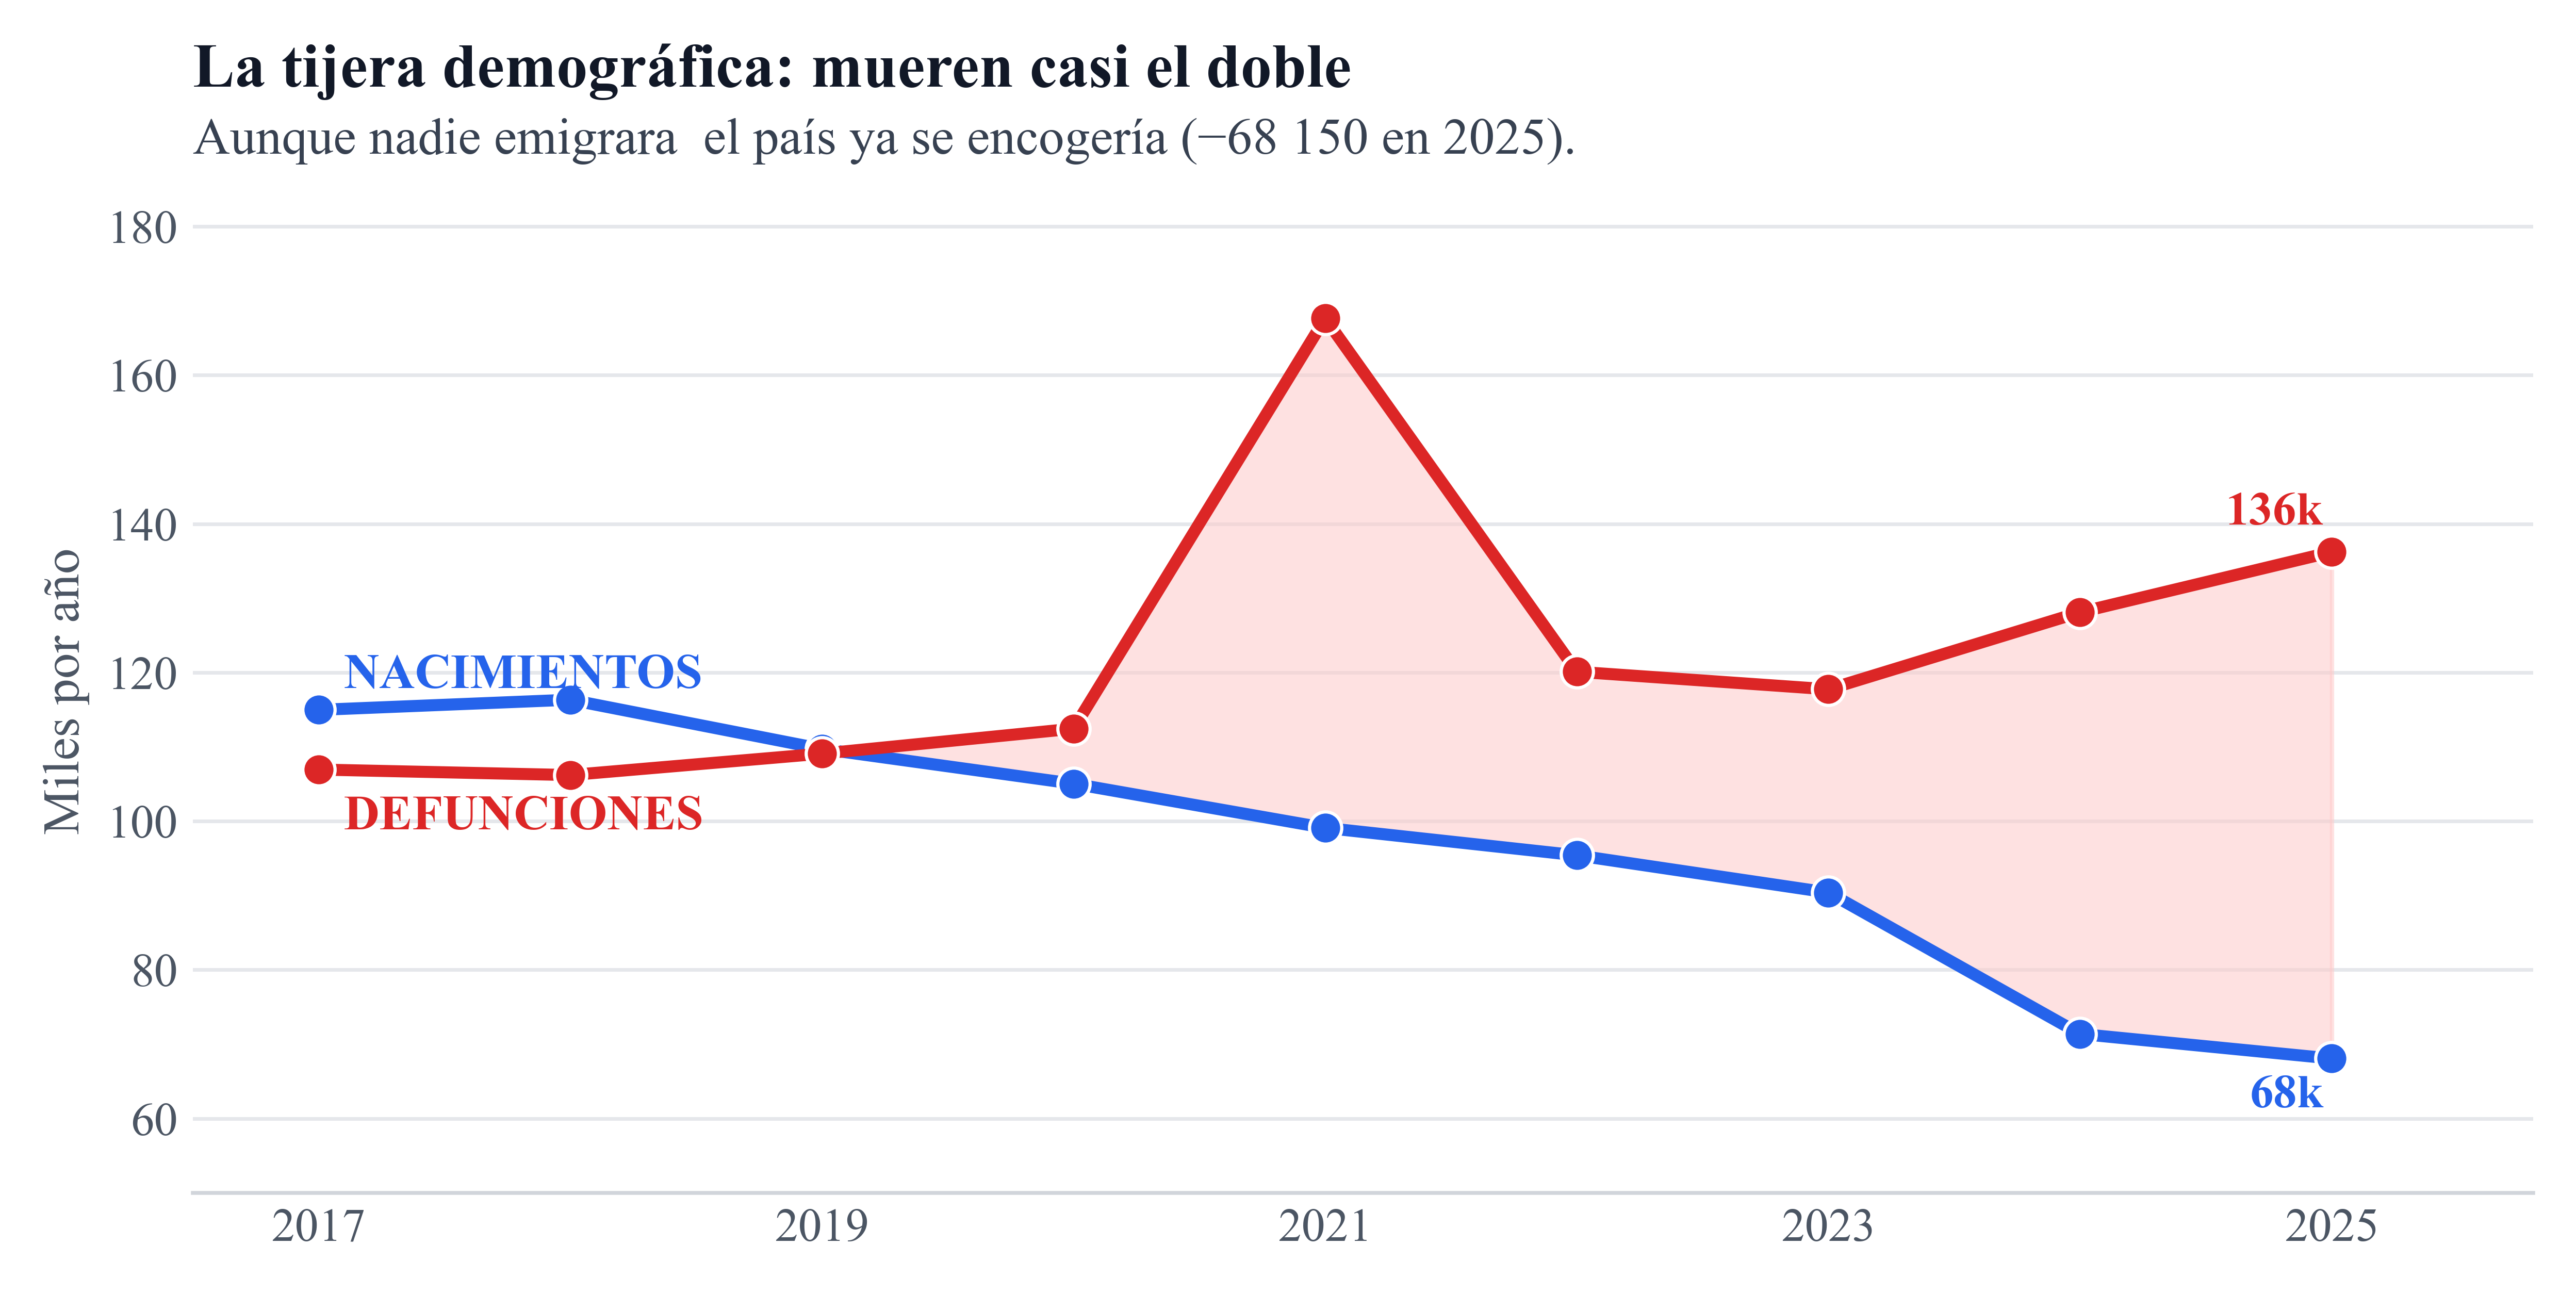
\includegraphics[width=\linewidth]{f2_tijera_es.png}
\caption{Nacimientos frente a defunciones (``la tijera''): las defunciones duplican a los nacimientos en 2025.}
\label{fig:scissors}
\end{subfigure}\hfill
\begin{subfigure}[t]{0.495\linewidth}
\centering
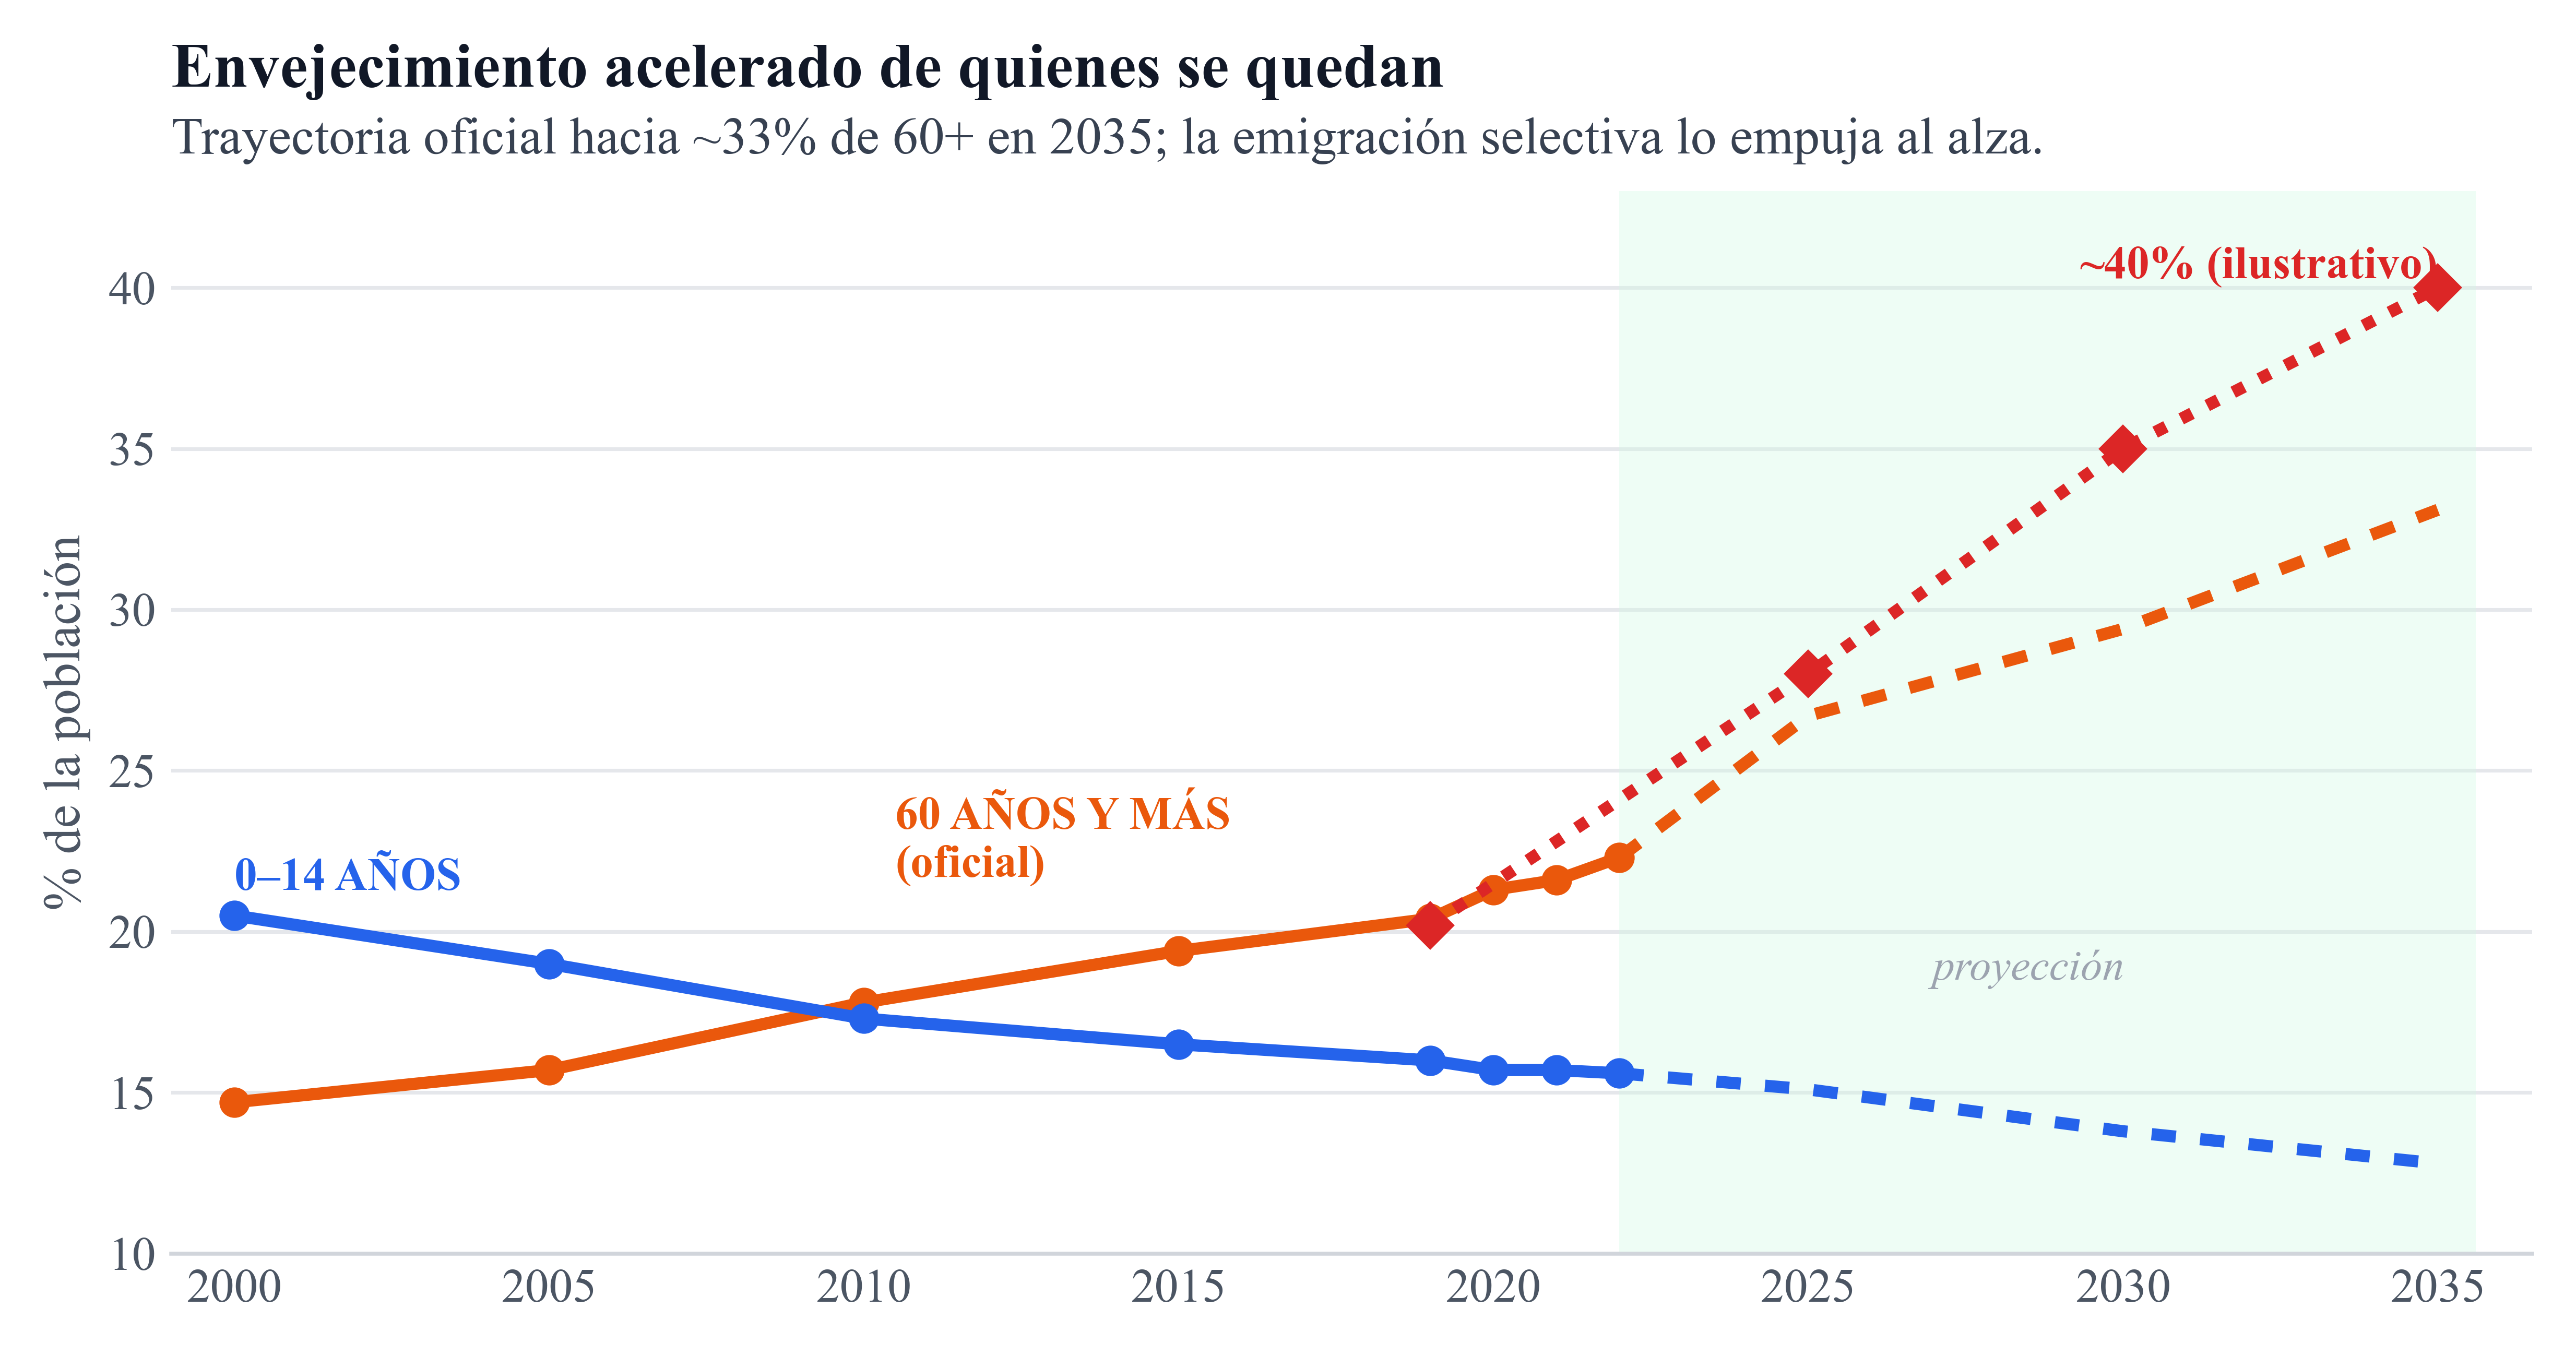
\includegraphics[width=\linewidth]{f4_envejece_es.png}
\caption{Envejecimiento acelerado a medida que se van los adultos en edad laboral (estructura oficial).}
\label{fig:aging}
\end{subfigure}
\caption{Motor demográfico interno: decrecimiento natural y envejecimiento acelerado.}
\label{fig:internal}
\end{figure}

La esperanza de vida al nacer oficial alcanzó su máximo en 2011--13 (78.5 años) y bajó a 77.7 en 2018--20; una estimación independiente de 2021 la sitúa cerca de 71 años~\citep{albizu2023,bronnum2023}.
Esa caída es grande frente a las pérdidas internacionales de la era COVID~\citep{aburto2022,msemburi2023}; la esperanza de vida reexpresa la mortalidad en lugar de corroborar de forma independiente el escenario central (series en el suplemento (en inglés)).
Las defunciones infantiles subieron de 461 (2018) a 715 (2022); la tasa alcanzó 9.9 por mil en 2025 ($+$98\% desde 2019).

La descomposición de la mortalidad responde directamente a la pregunta envejecimiento frente a colapso (Figura~\ref{fig:attrib}).
Cuba registró 136\,214 defunciones en 2025 frente a 109\,080 en 2019 ---27\,134 más, o unas 31\,300 una vez añadidas las defunciones no registradas estimadas--- mientras el stock del escenario central es unos 2~millones menor (la serie oficial cae 1.76~millones en el mismo tramo).
Entretanto, la población de 60 años y más subió de 2.31~millones (2019, observado) a unos 2.60~millones proyectados en 2025.
Tres términos dan cuenta de ese aumento (las medianas no son aditivas, de modo que suman 31\,500 y no 31\,300).
Una población residente menor en $\sim$2~millones debería haber reducido las defunciones anuales en unas \textbf{19\,400}; el envejecimiento añadió unas \textbf{22\,400}; y el residual de exceso respecto de la tabla de 2019 es de unas \textbf{28\,500} al año (rango de sensibilidad a los supuestos: 18\,600--38\,200), o $\sim$297 por cada 100\,000 sobre la población oficial.
Los dos términos al alza son de magnitud comparable ($\sim$44\% y $\sim$56\% del incremento bruto); ninguno por sí solo explica el aumento, y juntos lo superan porque la población menguante tira en sentido contrario.
El puente basado en tasas brutas reportado en versiones anteriores de este trabajo cargaba a la crisis todo el desplazamiento etario y sobrestimaba el componente de colapso: $\sim$77\,000 para 2024--2025 combinados frente a \textbf{50\,100} (32\,600--67\,500) aquí.

El perfil temporal separa dos episodios distintos.
El exceso respecto de la tabla de 2019 fue de unas 5\,400 en 2020, alcanzó $\sim$61\,900 en la ola de COVID-19 de 2021, retrocedieron a $\sim$12\,800 (2022) y $\sim$11\,900 (2023), y luego casi se duplicaron hasta $\sim$21\,600 (2024) y $\sim$28\,500 (2025).
El valle de 2022--2023 separa la ola pandémica del alza posterior, de modo que el aumento de 2024--2025 no es una continuación del pico de 2021; coincide con las crisis de apagones, combustible, medicamentos y arbovirosis, aunque el residual por sí solo no permite descartar la mortalidad pos-aguda por COVID-19 ni cambios de codificación como contribuyentes.
Excluyendo 2021 por completo, el total de exceso de 2022--2025 es de $\sim$\textbf{74\,800} (47\,000--103\,000); incluyéndolo, 2020--2025 da $\sim$142\,100 (105\,400--180\,500).
Una continuación de escenario para 2026 llega a $\sim$32\,300 (20\,000--44\,200), pero esa cifra hereda la continuación supuesta de $+$4\% en defunciones y no es una observación.
La incertidumbre dominante no está dentro de la simulación sino en la elección del contrafactual, y no está en el rango anterior.
Mantener plana la mortalidad de 2019 es un supuesto, y ajustamos la tendencia precrisis en lugar de afirmarla. El resultado es que \textbf{la tendencia no es identificable}: la serie dispersa 2006--2019 (cuatro años son inutilizables, véanse las Advertencias) da $+0.236\%$/año ($p=0.066$, IC 95\% $-0.02$ a $+0.49$) y la ventana contigua 2013--2019 da $+0.678\%$/año ($p=0.064$, IC $-0.06$ a $+1.41$). Ambos intervalos contienen el cero. Por eso \emph{no} ajustamos la tendencia ni la propagamos, lo que fabricaría una precisión que la serie no sostiene; el ancla plana es una convención declarada, no un hallazgo. La sensibilidad siguiente usa en consecuencia los límites que los datos permiten y no las estimaciones puntuales: el límite superior de la ventana más inclinada ($+1.41\%$/año) da 18\,500 para 2025, y la mejora del 0.5--1.5\%/año de los pares regionales da 31\,600--38\,000.
El rango completo, \textbf{18\,500--38\,000}, es \emph{más amplio} que el rango reportado y no se propaga a él. El mismo ejercicio sobre la ventana acumulada mueve 2022--2025 de 74\,200 a \textbf{45\,200--103\,300}, de modo que los 74\,800 del resumen dependen del ancla plana del mismo modo. Esto, y no nada interno a la simulación, es la medida honesta de cuán bien se conoce esta cantidad. Un ancla plana tiende más a subestimar que a sobrestimar, porque los pares regionales de Cuba siguieron mejorando.
Pasando al ruido interno del ancla y no a su elección: las tasas por edad promedio de 2017--2019 quedan a menos del 1.1\% de las de 2019 a los 65 años y más, donde ocurre la mayoría de las defunciones, y ligeramente \emph{por encima}, de modo que 2019 fue un año comparativamente bueno y el ancla no favorece el resultado; la diferencia queda holgadamente dentro del ruido del 2\% de la tabla de tasas.

\begin{figure}[!htbp]
\centering
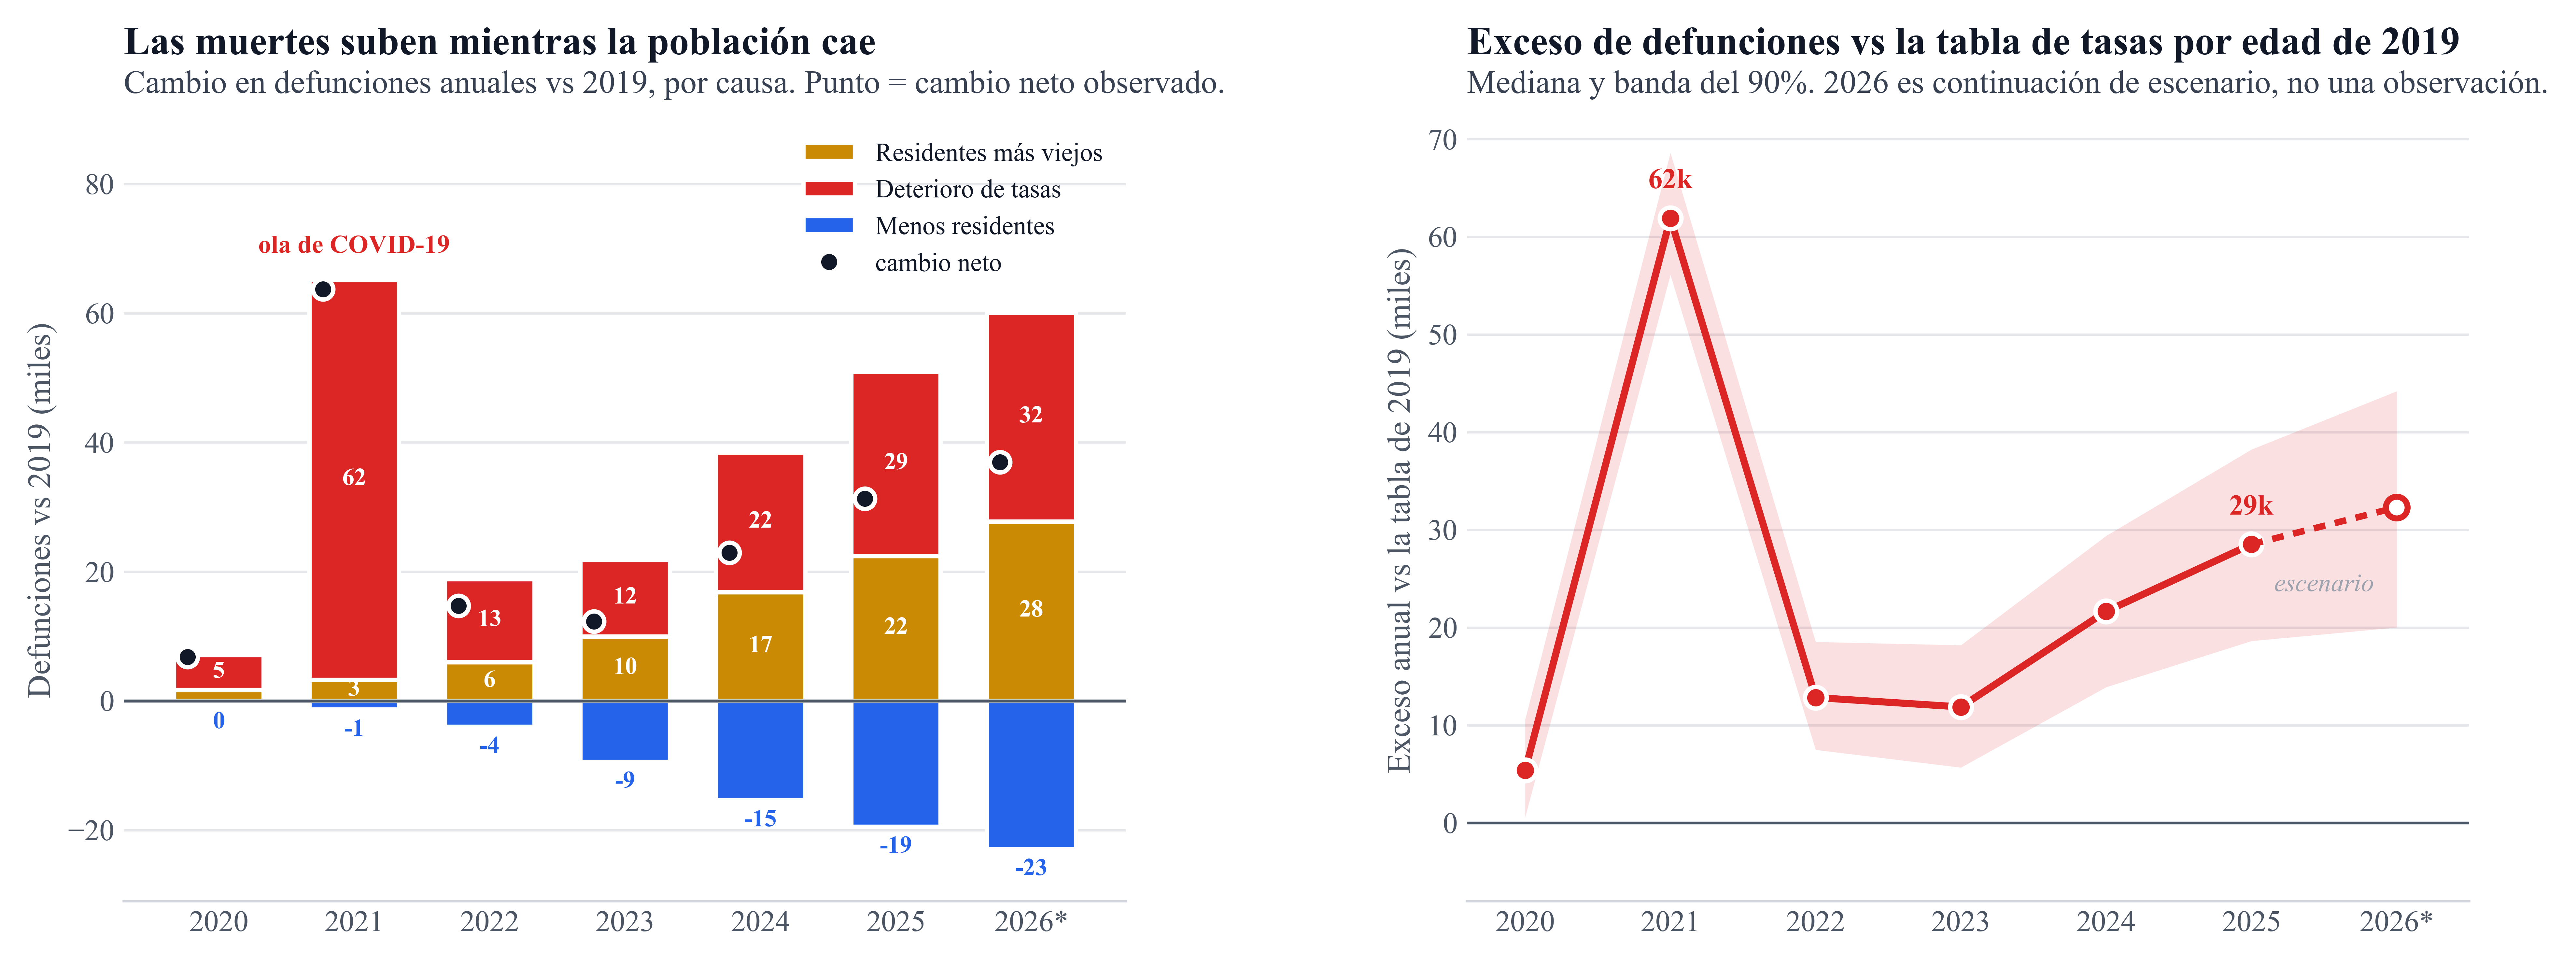
\includegraphics[width=\linewidth]{f14_atribuible_es.png}
\caption{Por qué suben las defunciones mientras cae la población.
Izquierda: cambio en las defunciones anuales frente a 2019, descompuesto en tamaño poblacional, envejecimiento y deterioro de tasas; el punto es el cambio neto observado incluidas las defunciones no registradas estimadas.
Derecha: defunciones de exceso respecto de la tabla de 2019, mediana y rango de sensibilidad a los supuestos.
2026 es una continuación de escenario, no una observación.
Las bandas son predictivas a priori bajo las marginales indicadas y comparten $D_{\mathrm{fac}}$ con el escenario central.}
\label{fig:attrib}
\end{figure}

\subsection{Población proyectada}

Las fuentes que no depuran emigrantes (padrón electoral, denominador de salud del MINSAP) quedan altas y funcionan como techos blandos.
Las construcciones que corrigen por salida (ocupación de viviendas $\sim$8.7~M; Albizu-Campos 8.0--8.6~M) quedan cerca del escenario central pero comparten con este estudio los supuestos de crítica migratoria; no son censos independientes.
El oficial de 9.43~M queda entre ambas familias (Figura~\ref{fig:tri}).
La participación electoral cayó abruptamente entre 2018 y 2023; ese patrón es compatible con ausencia física pero también con abstención, logística y factores políticos, y \emph{no} se usa como recuento de personas.

\begin{figure}[!htbp]
\centering
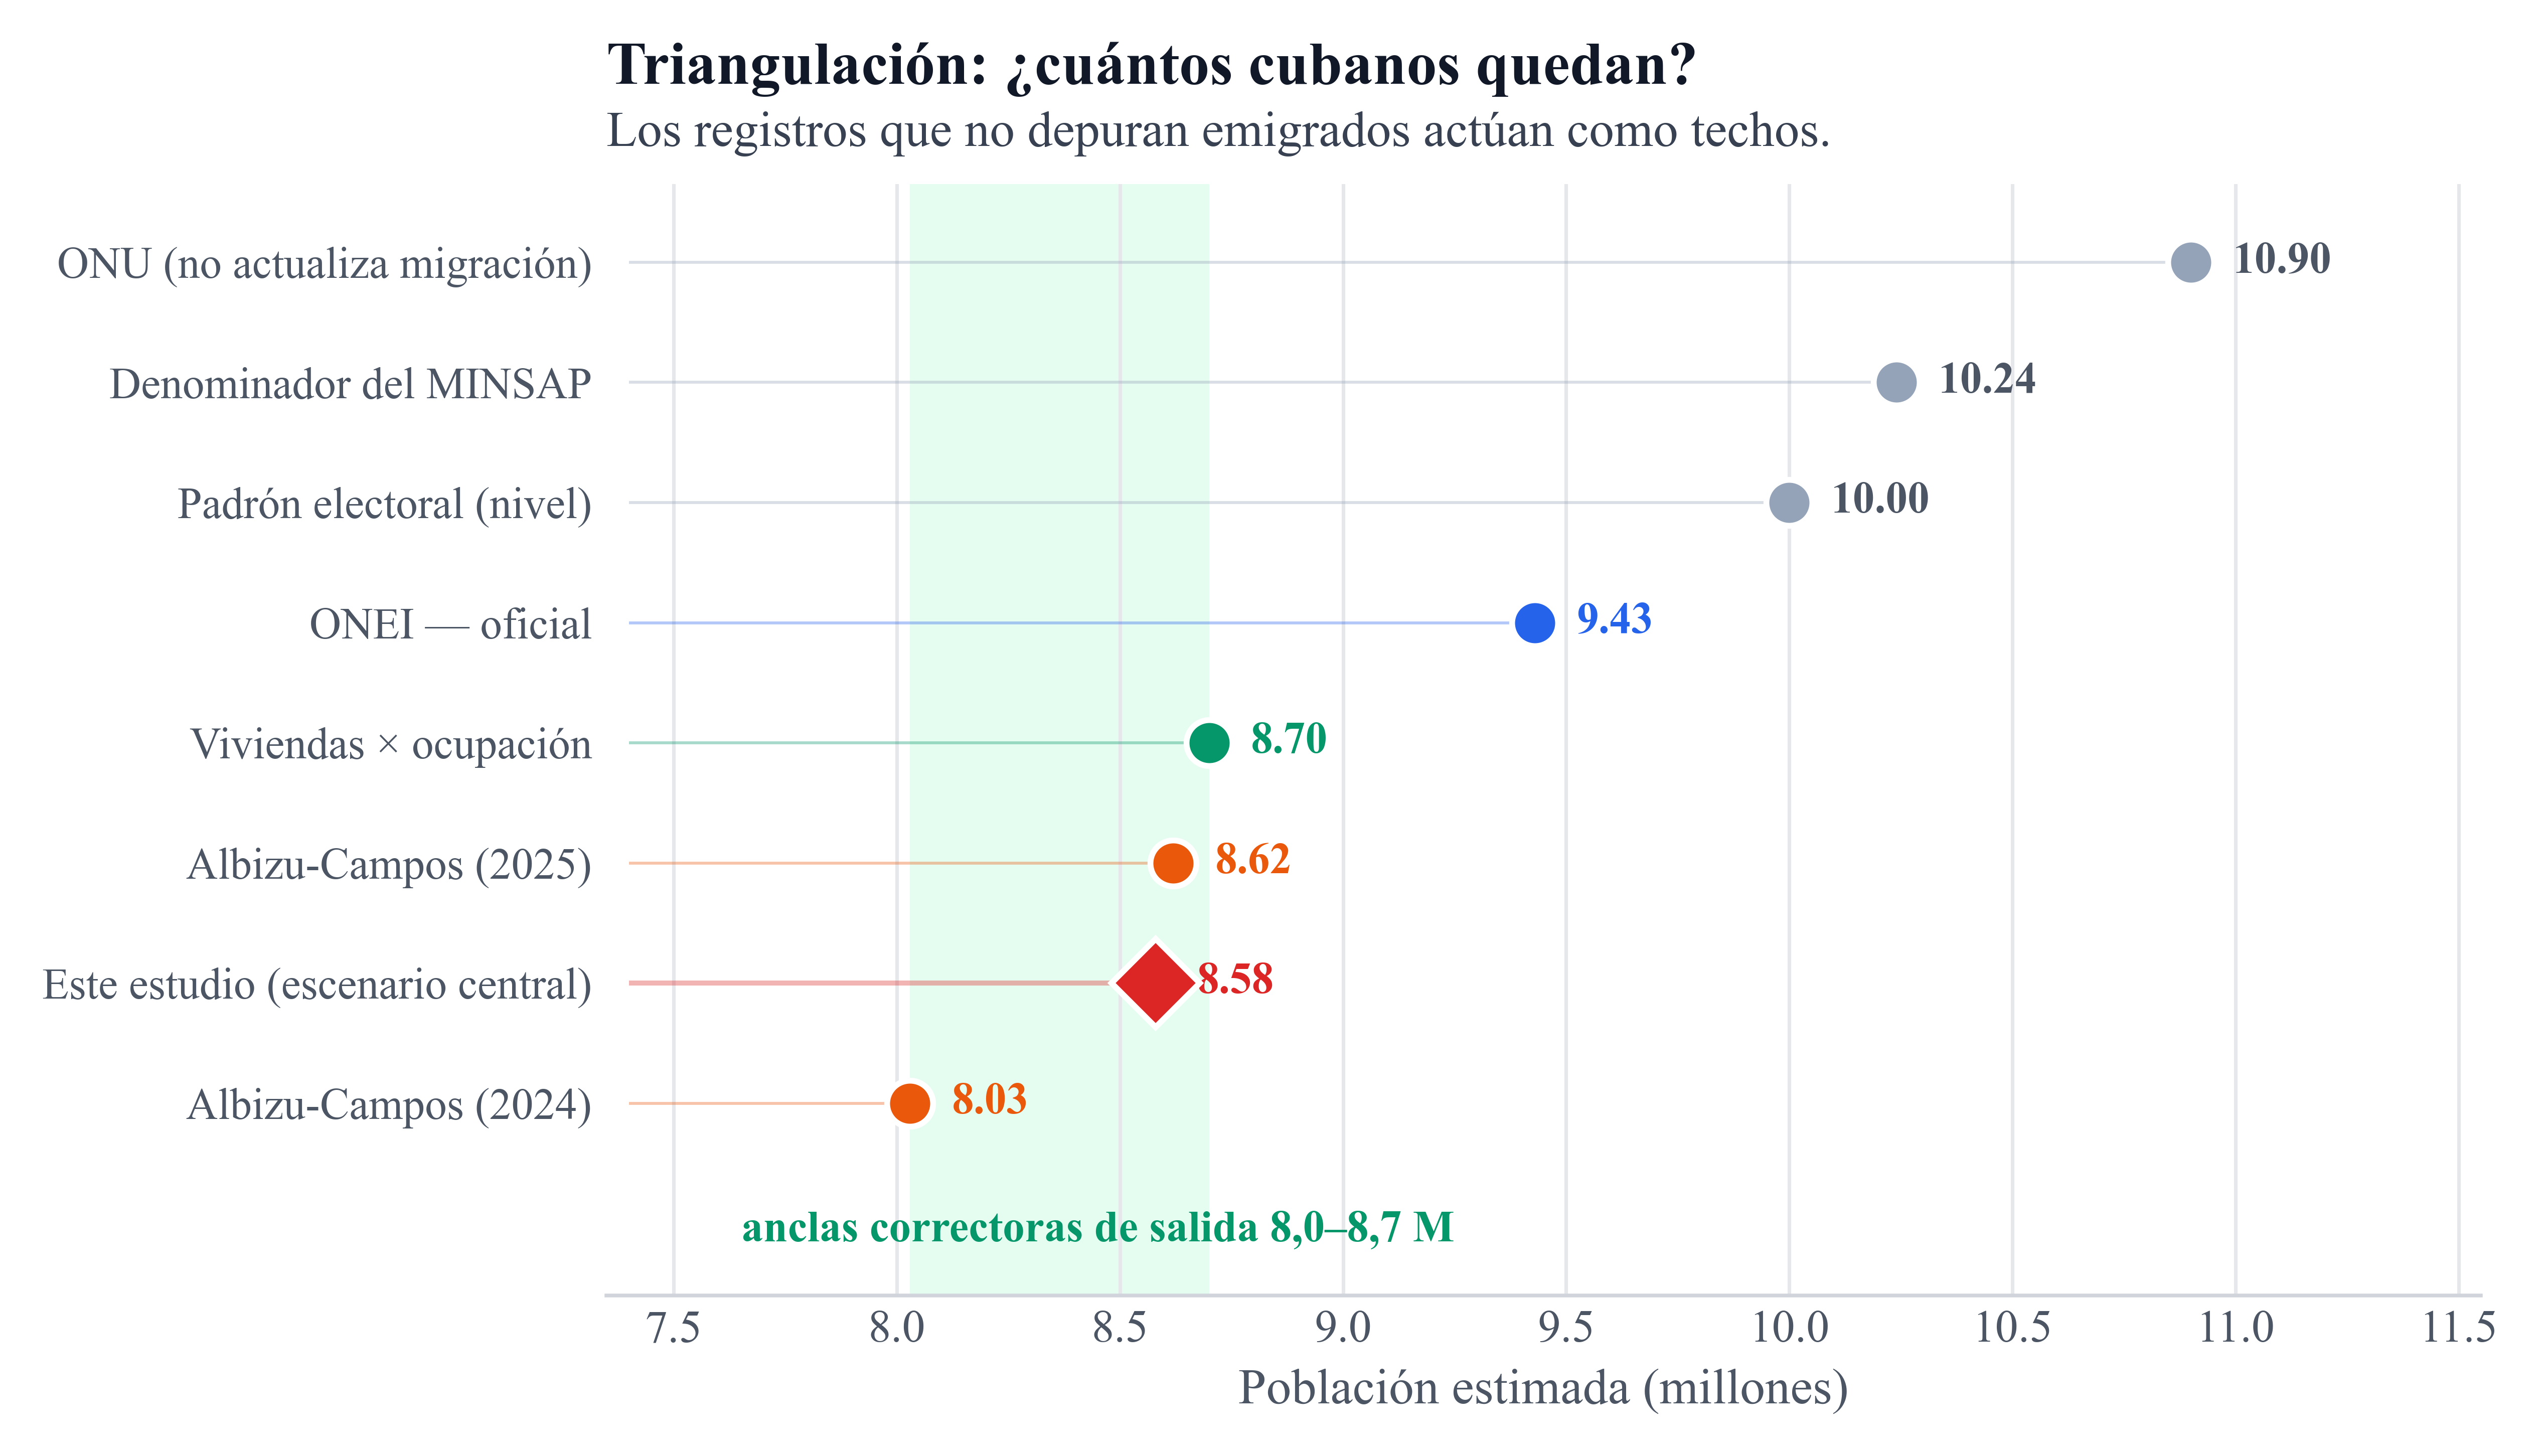
\includegraphics[width=0.95\linewidth]{f7_triangulacion_es.png}
\caption{Triangulación de los niveles de población a fin de 2025.
El escenario central es el estimando del estudio (no un validador); Albizu y viviendas son anclas blandas y cargadas de supuestos.}
\label{fig:tri}
\end{figure}

El Cuadro~\ref{tab:models} resume los tres escenarios.
El enunciado primario de incertidumbre es la envolvente entre escenarios: frente al stock oficial de fin de 2021 (11.11~millones), la brecha a fin de 2025 abarca \textbf{1.97--2.79~millones}, o \textbf{17.8--25.1\%}.
El escenario central sitúa la población viva en \textbf{8.58~millones} (brecha \textbf{2.53~millones}, \textbf{22.8\%}) frente a 9.43~millones oficiales, con el piso en 9.14~millones y el caso superior en 8.32~millones.
La emigración explica alrededor del \textbf{92\%} de la brecha central una vez contado el rezago previo a 2021 junto al flujo de 2022--2025; dentro del flujo solo, $\sim$91\%.
La continuación a fin de 2026 sitúa el escenario central cerca de \textbf{8.29~millones} (envolvente 8.02--8.84~millones).
Al haber ahora una sola base, el titular tiene una sola forma: entre aproximadamente una de cada seis y una de cada cuatro personas contadas oficialmente en 2021 no está.

\begin{table}[ht]
\centering
\caption{Tres escenarios sobre una sola base: el stock oficial de fin de 2021 (11\,113\,215).
Las estimaciones puntuales son de forma cerrada; las bandas del 90\% dentro de cada escenario son dispersiones predictivas a priori No son intervalos de confianza, no tienen propiedad de cobertura, y ningún parámetro de este trabajo se informa con una verosimilitud.
Versiones anteriores llevaban cinco conjuntos de priores; una variante ajustada por crisis (a 0.02~M del central) y un acompañante de reconstrucción vital se han retirado.}
\label{tab:models}
\begin{tabular}{lrrrr}
\toprule
Escenario & Brecha (M) & Brecha \% & Pob.\ fin-2025 (M) & Pob.\ fin-2026 (M) \\
\midrule
\textit{Nulo: ONEI al pie de la letra} & \textit{1.68} & \textit{15.1} & \textit{9.43} & \textit{9.14} \\
Conservador & 1.97 & 17.8 & 9.14 & 8.84 \\
\textbf{Central ajustado por crisis} & \textbf{2.53} & \textbf{22.8} & \textbf{8.58} & \textbf{8.29} \\
Superior de estrés & 2.79 & 25.1 & 8.32 & 8.02 \\
\midrule
\textit{Envolvente (excl.\ nulo)} & \textit{1.97--2.79} & \textit{17.8--25.1} & \textit{8.32--9.14} & \textit{8.02--8.84} \\
\bottomrule
\end{tabular}
\end{table}

\begin{figure}[!htbp]
\centering
\begin{subfigure}[t]{0.495\linewidth}
\centering
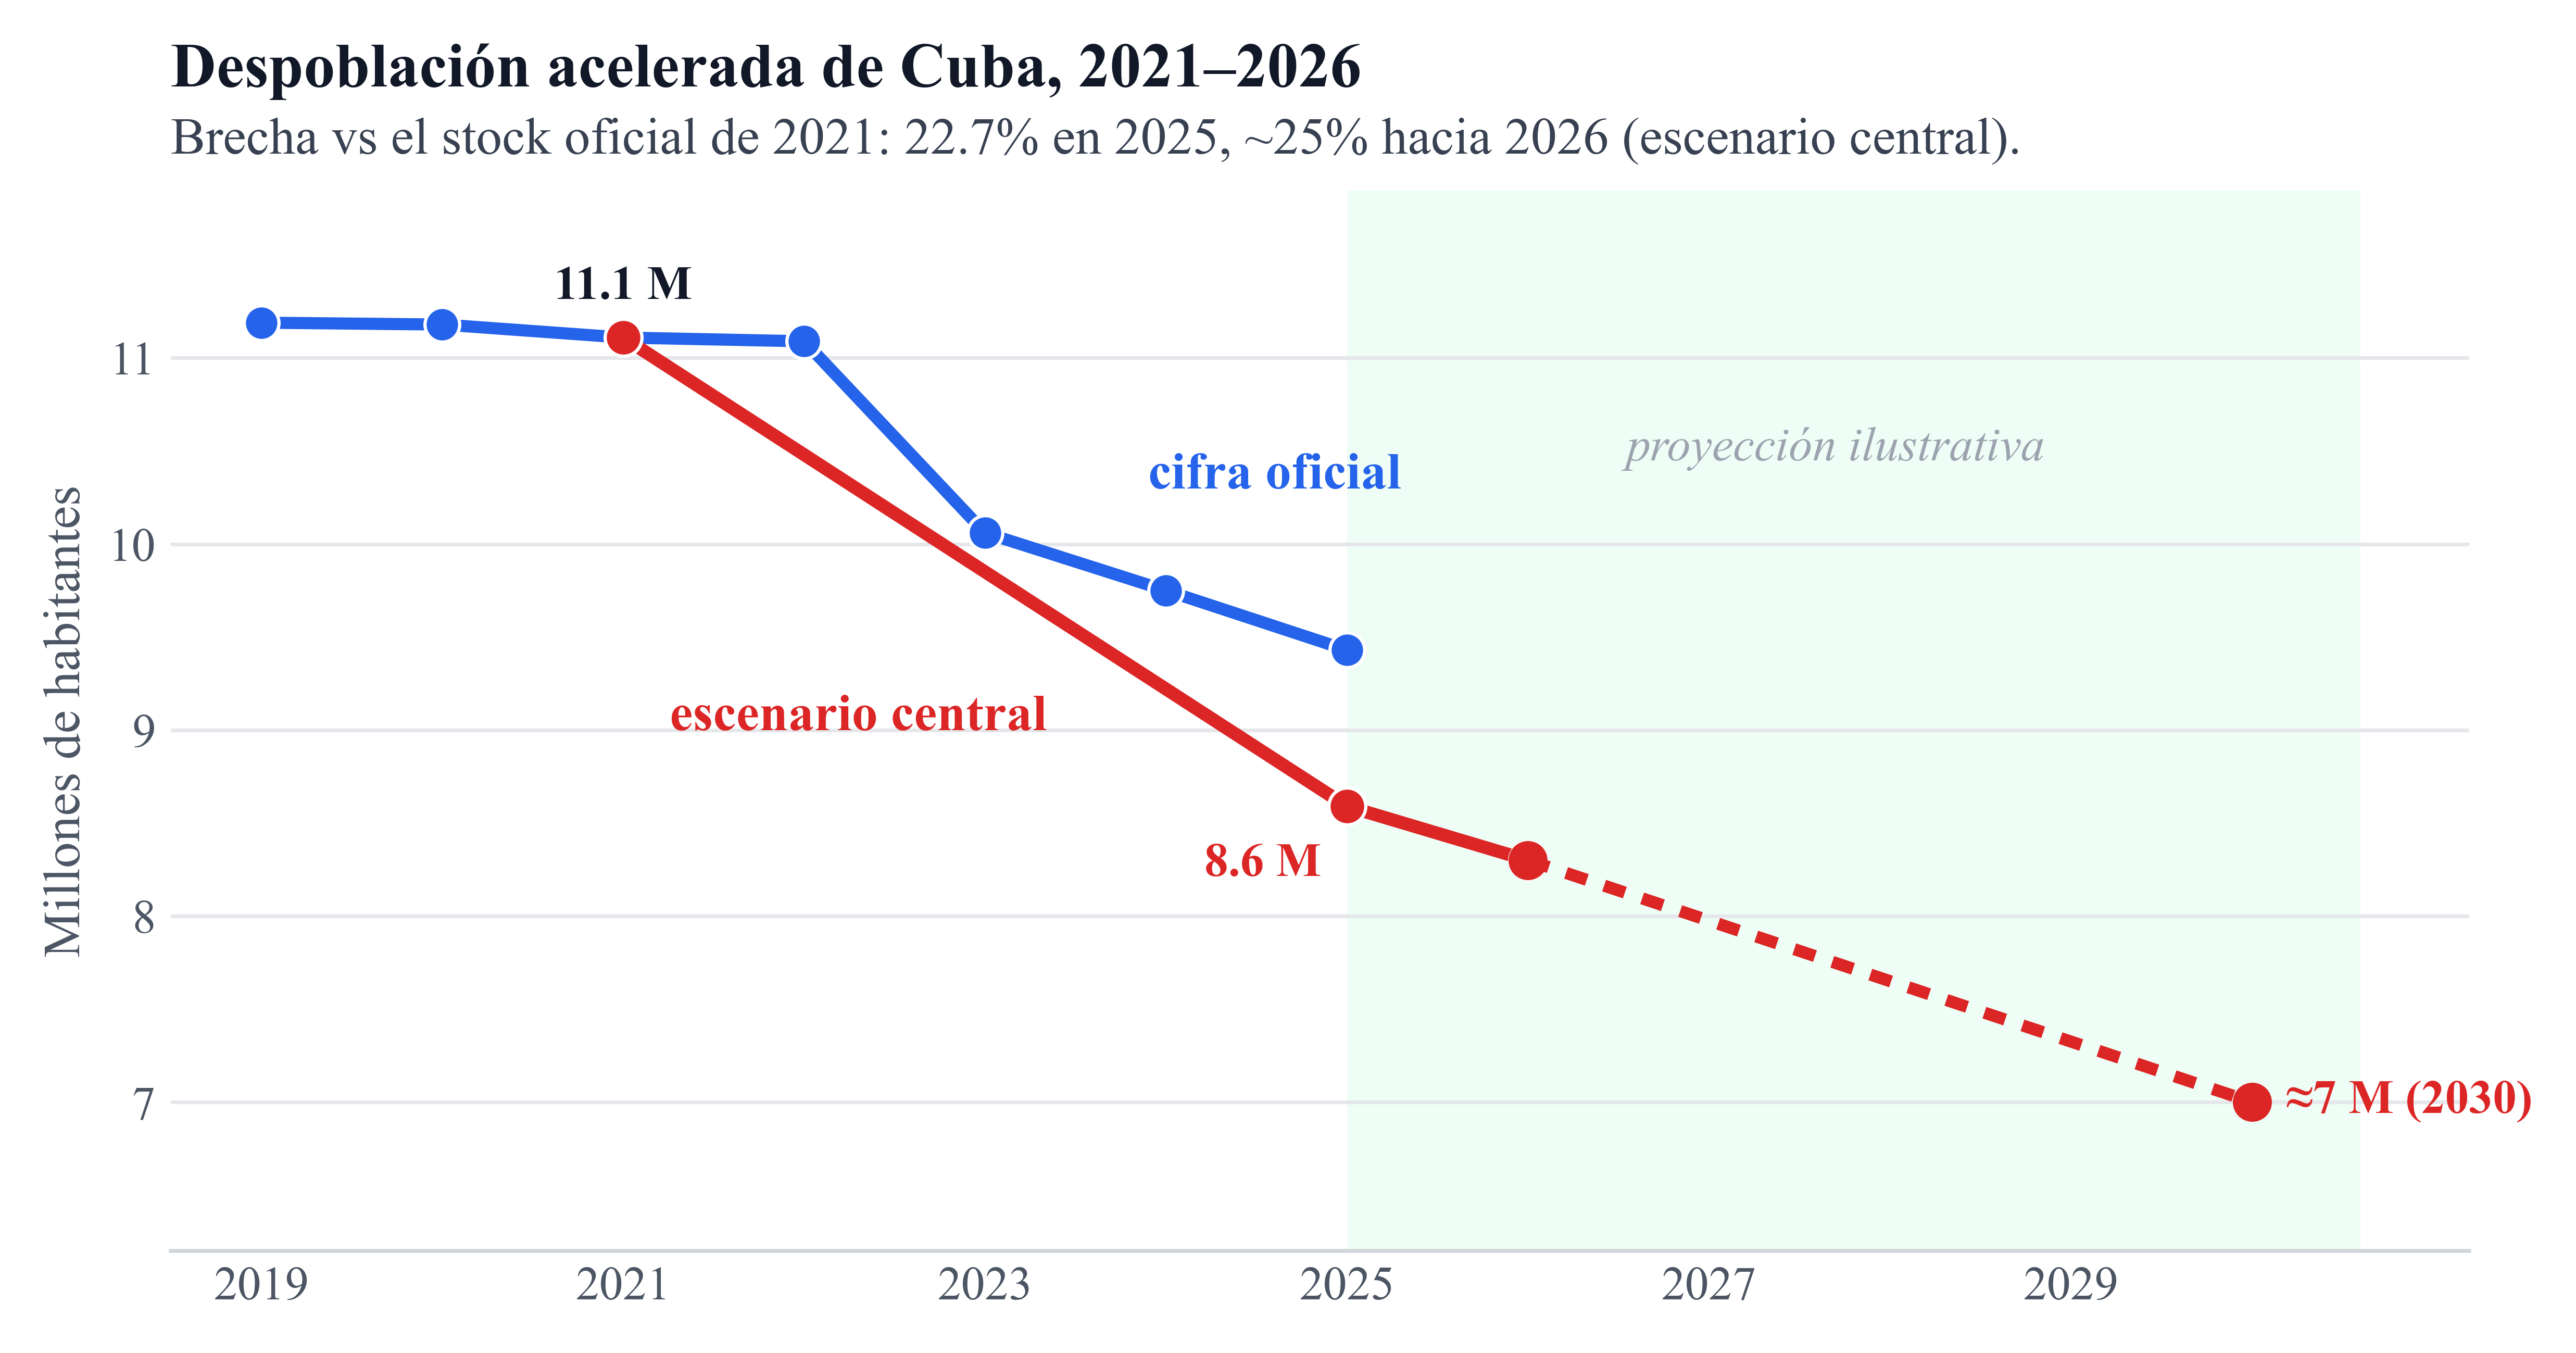
\includegraphics[width=\linewidth]{f1_poblacion_es.png}
\caption{Población oficial frente a población viva por escenario, 2021--2030 (trayectoria ilustrativa del escenario central en rojo; el tramo posterior a 2026 es un escenario de tendencia no probabilístico).}
\label{fig:pop}
\end{subfigure}\hfill
\begin{subfigure}[t]{0.495\linewidth}
\centering
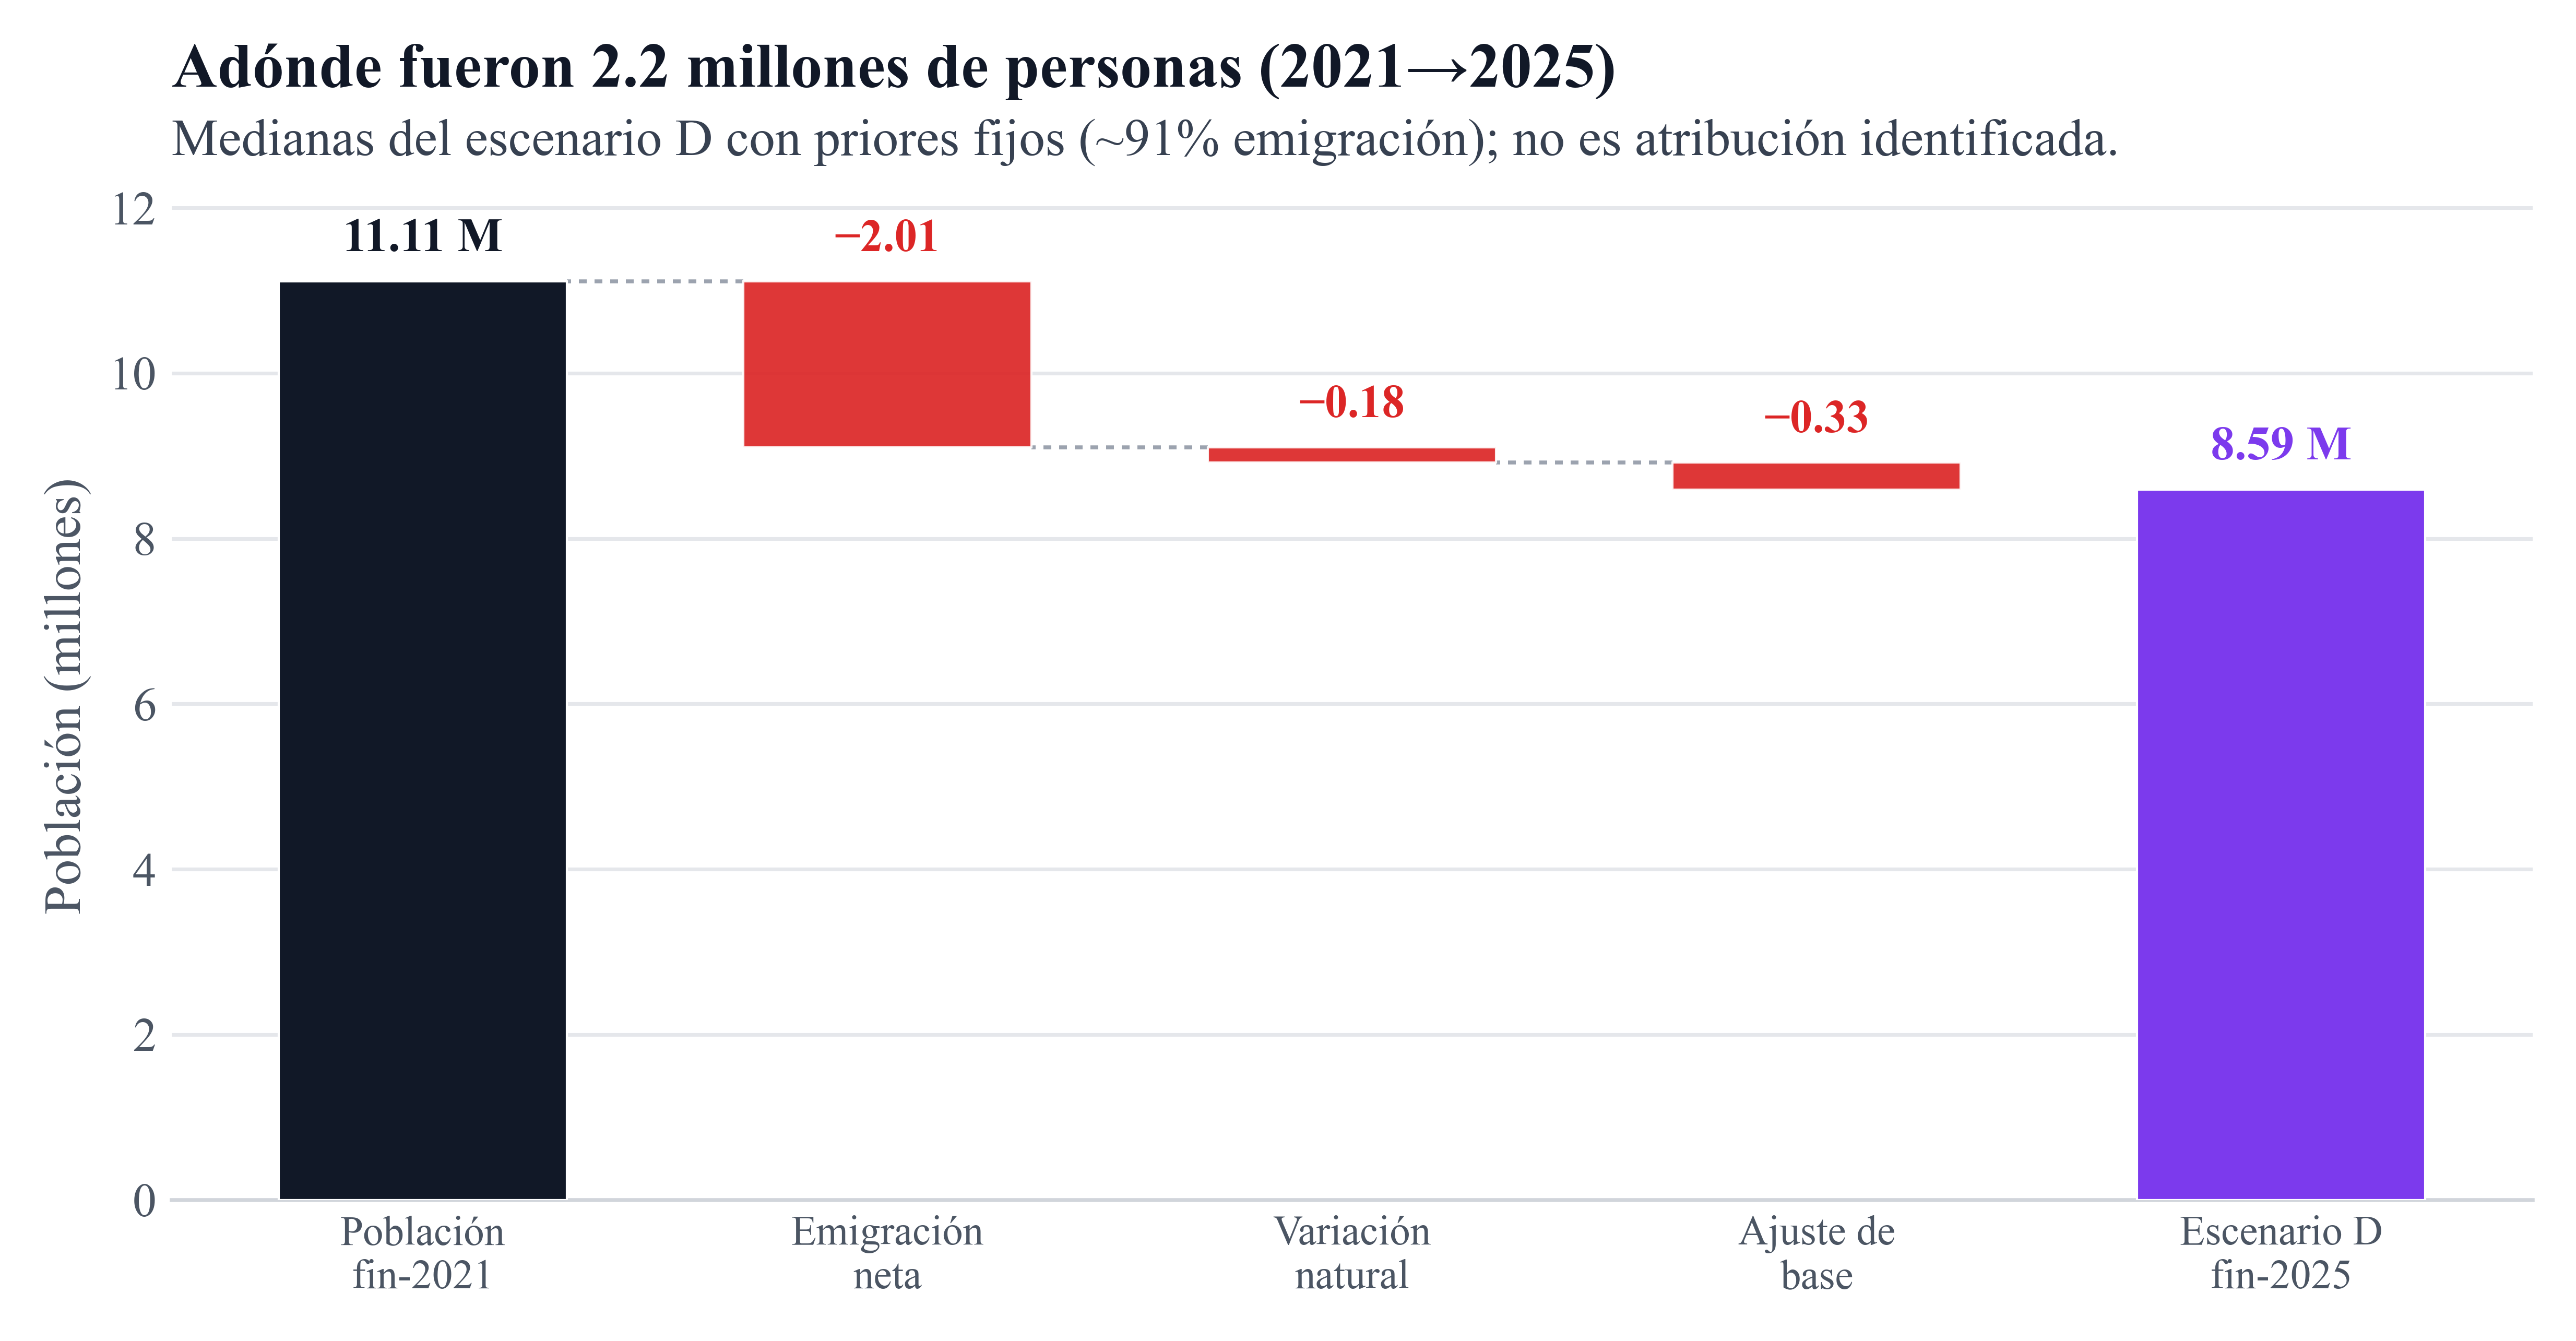
\includegraphics[width=\linewidth]{f3_cascada_es.png}
\caption{Descomposición contable con medianas del escenario central (2021--2025); escenario ilustrativo, no una atribución identificada.}
\label{fig:cascade}
\end{subfigure}
\caption{Trayectoria poblacional principal y descomposición contable.}
\label{fig:headline}
\end{figure}

En el plano regional, América Latina y el Caribe todavía crecen ($\sim$+$0.7\%$ anual; Cuadro~\ref{tab:region}, aproximaciones de WPP de la ONU y CEPAL).
Cuba muestra una pérdida neta de población de alrededor de $-$3.3\% anual en comparaciones sobre la trayectoria oficial reciente.
Entre las contracciones en tiempos de paz impulsadas por la emigración, Venezuela es el par regional más cercano (Cuadro~\ref{tab:hist}); los casos impulsados por desastres no se tratan como pares.
Hacia \textbf{fin de 2026}, la continuación central implica una pérdida adicional de unas 300\,000 personas: población viva cerca de \textbf{8.29~millones} (banda entre escenarios 8.02--8.84~M).
Hacia fin de 2026 el escenario superior alcanza una brecha de $\sim$3.1~millones y el central $\sim$2.8~millones ($\sim$25\%).
Las trayectorias de tendencia ilustrativas hacia $\sim$7~millones en 2030 (Figura~\ref{fig:pop}, tramo posterior a 2026) son solo escenarios.

\begin{table}[ht]
\centering
\caption{Cuba frente a contracciones seleccionadas impulsadas por la emigración en tiempos de paz.
La fila de Cuba usa el escenario central sobre la base oficial de 2021; los comparadores son aproximados y no están armonizados por ventana temporal. La fila de Puerto Rico está confundida por el desastre del huracán María.}
\label{tab:hist}
\begin{tabular}{lrrr}
\toprule
Caso & Pérdida acum. & Anual aprox. & Motor dominante \\
\midrule
Venezuela 2013--24 & $\sim$25\% & 1--3\% & emigración \\
Puerto Rico post-2017 (era Mar{\'i}a) & salida neta grande & --- & emigración + desastre \\
Cuba 2021--25 (central) & $\sim$22.8\% (base oficial) & $\sim$3--5\% & emigración + interno \\
\bottomrule
\end{tabular}
\end{table}

\begin{table}[ht]
\centering
\caption{Crecimiento poblacional anual: Cuba frente a la región (aproximado; revisión 2024 de WPP de la ONU y CEPAL, redondeado).}
\label{tab:region}
\begin{tabular}{lr}
\toprule
País / región & Crecimiento anual \\
\midrule
Guatemala & $+1.7\%$ \\
Bolivia & $+1.4\%$ \\
República Dominicana & $+1.0\%$ \\
México & $+0.8\%$ \\
Colombia & $+0.7\%$ \\
\textit{América Latina y el Caribe} & $+0.7\%$ \\
Brasil & $+0.4\%$ \\
Chile & $+0.3\%$ \\
Uruguay & $+0.1\%$ \\
Venezuela & $\approx 0\%$ (tras $\sim$25\% de pérdida 2013--24) \\
Cuba & $-3.3\%$ \\
\bottomrule
\end{tabular}
\end{table}

\section{Discusión}

\subsection{Migración}



El único caso documentado de revisión a la baja del registro de defunciones es ilustrativo.
Usamos la cifra publicada, pero el total previo a la revisión elevaría la mortalidad en exceso de 2022 de $\sim$12\,700 a $\sim$21\,900, y el total pospandémico 2022--2025 de $\sim$74\,800 a $\sim$84\,100.
Este es el anclaje empírico de cuánta holgura tiene demostrablemente el registro: un 7.5\% en un solo año, apenas por debajo del tope del 9\% sobre $D_{\mathrm{fac}}$, razón por la cual ese tope se mantiene en lugar de elevarse.
Acota la pregunta desde la observación y no desde una creencia previa, y corta en ambas direcciones: un registro que puede perder 8\,951 defunciones sin explicación no es plenamente confiable, pero uno que publicó un alza del 54\% en un solo año en 2021 (de 109\,080 a 167\,645) tampoco es uno que oculte a gran escala.

El saldo migratorio declarado por la ONEI para 2022 ($+$991) es incompatible con cientos de miles de llegadas de cubanos a Estados Unidos ese mismo año bajo cualquier conversión plausible de encuentros a emigrantes (los encuentros no son emigrantes netos únicos en proporción 1:1).
Buena parte del éxodo se contabiliza en una sola revisión de 2023, compatible con una puesta al día rezagada del registro asentada en un único año.
Incluso tras esa revisión, los saldos netos de 2024--2025 quedan solo ligeramente por encima de las entradas registradas únicamente en Estados Unidos, mientras que el saldo de 2025 admite 317\,320 emigraciones externas brutas (neto $-$245\,264): un déficit frente al piso multidestino, aunque el saldo de 2025 es internamente consistente.
Por eso este trabajo trata el recuento oficial como un techo y lo contrasta con fuentes que corrigen por salida (Figura~\ref{fig:tri}).

En conjunto: frente al stock oficial de fin de 2021, la brecha a fin de 2025 se sitúa entre 1.97 y 2.79~millones, o 17.8--25.1\% (el enunciado primario).
Bajo el escenario central, la población viva está cerca de 8.58~millones a fin de 2025 y no en los 9.43~millones oficiales: una brecha de 2.53~millones (22.8\%), de la cual alrededor del 92\% es emigración; el piso anclado en la ONEI queda en 9.14~millones.
Hacia fin de 2026 la continuación central está cerca de 8.29~millones, llevando la brecha a aproximadamente una de cada cuatro personas.
Junto a ese recuento ---de cuya brecha de 2.53~millones, 1.68~millones son caída ya publicada por la ONEI y 0.85~millones la corrección de este trabajo--- el exceso respecto de la tabla de 2019 corre a $\sim$28\,500 defunciones al año a niveles de 2025 y a $\sim$74\,800 acumuladas en 2022--2025, un costo mayor que lo que explica el envejecimiento por sí solo y alrededor de un tercio inferior a lo que implicaba para 2024--2025 el puente basado en tasas brutas.
Un censo en 2026 realizado con prácticas estándar sería informativo; la banda de escenario de trabajo a fin de 2026 es de 7.9--8.9~millones y no la trayectoria de 10.9~millones de \emph{World Population Prospects} bajo supuestos de emigración neta todavía bajos~\citep{un_wpp}.


\subsection{Deterioro del sistema de salud}

Los dos motores se encuentran en la descomposición de la mortalidad, y leerla correctamente importa.
La emigración se lleva adultos en edad laboral, lo que eleva la proporción de ancianos, lo que a su vez eleva las defunciones incluso con un sistema de salud inalterado: eso es lo que mide el término de envejecimiento: unas 22\,400 defunciones adicionales al año.
Cuánto de ese envejecimiento es inducido por la migración \emph{no} se identifica aquí: el término se calcula sobre la estructura por edades observada de la ONEI, y la transición de la fecundidad cubana ya generaba envejecimiento décadas antes de la crisis, de modo que debe leerse como envejecimiento por todas las causas combinadas, de las cuales la salida selectiva es una.
Encima de él se sitúa un deterioro de tasas de $\sim$28\,500 defunciones al año que el envejecimiento no explica, concentrado en 2024--2025 y todavía en ascenso en el escenario de 2026.
La asimetría relevante para la política pública es que la emigración puede revertirse, mientras que ni esas muertes ni los nacimientos que no ocurrieron pueden hacerlo.
Dos propiedades hacen que la estimación de exceso sea más robusta que los escenarios poblacionales junto a los que se presenta: no depende de resolver la disputa migratoria, porque el número de ancianos se mantiene aproximadamente fijo y $E_t$ apenas se mueve entre la población oficial y la del escenario central; y es insensible al \emph{nivel} del ancla, que la sensibilidad 2017--2019 deja esencialmente inalterado a los 60 años y más (\emph{no} es insensible a su tendencia, que es la incertidumbre dominante señalada arriba).
Sigue siendo condicional a que el registro de defunciones sea casi completo: un supuesto que el centinela de mortalidad infantil hace plausible para las muertes institucionales pero no demuestra, y que la distribución a priori de $D_{\mathrm{fac}}$ pretende absorber más que resolver.
Su debilidad principal es la opuesta a la de los modelos poblacionales: el mecanismo no está identificado.
Los apagones, los fallos de ambulancias y de diálisis por falta de combustible, la escasez de medicamentos, la oncología demorada y las olas de arbovirosis de 2025--2026 son todas vías plausibles, y ninguna se estima aquí por separado; la estimación es una asociación con el período de crisis, no una atribución por causa de muerte.
Los indicadores de inseguridad alimentaria y anemia del PMA, y la caída del PIB agrícola, se discuten solo como vías \emph{contextuales} amplificadoras~\citep{wfp_cuba}; no entran en $D_{\mathrm{fac}}$ ni en la descomposición~\citep{karlinsky2021,msemburi2023}.


\subsection{Población proyectada}

El escenario central se mantiene porque la comprobación de consistencia con la mortalidad infantil reduce la necesidad de multiplicadores grandes de defunciones ocultas y concentra la incertidumbre residual en la migración~\citep{pagegarcia2020,modeld}.
No es una estimación puntual identificada: la pérdida absoluta sigue siendo $\sim$91\% migratoria bajo las distribuciones a priori del escenario central, y $U_0$ junto con $M>1$ pueden compartir un mismo defecto de padrón desactualizado.
Los intervalos dentro de un escenario parecen falsamente precisos frente a la envolvente entre escenarios: la envolvente debe encabezar la lectura.
El enunciado científico principal son los 0.85~millones en que el escenario central queda por debajo de la propia cifra de la ONEI para fin de 2025. La brecha de 2.53~millones (22.8\%) frente a la base oficial de 2021 es la suma de esa corrección y los 1.68~millones que la ONEI ya ha publicado; ambas no deben citarse indistintamente.
La salida es selectiva por edad y sexo; envejece la isla y deprime estructuralmente la fecundidad~\citep{coleman2006,diazbriquets2014,lee2014}.
El saldo natural, positivo en 2019, cayó a $-$68\,150 en 2025.

\section{Advertencias y limitaciones}

\textbf{Limitaciones.}
No hay censo desde 2012; la regla de $\sim$24 meses de la ONEI para contabilizar emigrantes rezaga las salidas recientes; los microdatos de destino son incompletos; los totales administrativos de ``asentados'' en Estados Unidos no son el stock de la ACS; los supuestos de ocupación de viviendas son frágiles; los bosquejos de envejecimiento no son proyecciones por componentes de cohorte; la esperanza de vida reexpresa la mortalidad; las trayectorias 2026--2030 son escenarios.
$U_0$ y $M$ pueden contar dos veces el rezago del padrón; los techos de encuentros en destino pueden inflar el número de personas únicas; los intervalos dentro de un escenario dan una falsa precisión frente a la incertidumbre estructural.
La descomposición de la mortalidad usa cuatro grupos de edad porque es el conjunto más fino que comparten los cuadros 3.15 y 3.3 de la ONEI; ambos se detienen en 2022, de modo que la estructura por edades de 2023--2026 es una proyección por cohortes y no una observación, y la composición dentro del grupo de 65 y más después de 2022 entra como un parámetro residual de deriva.
Su ancla de 2019 supone que no habría habido mejora contrafactual de la mortalidad cubana después de 2019, y comparte $D_{\mathrm{fac}}$ con el escenario central, por lo que no es independiente del escenario de recuento.
Las defunciones atribuibles son una asociación con el período de crisis, no una atribución por causa de muerte.
Los indicadores de inseguridad alimentaria son solo contextuales.

La serie precrisis estandarizada por edad no puede ajustarse sobre una ventana completa: los paneles de la ONEI 3.15 para 2009--2012 se leen como aproximadamente la mitad de las defunciones reales y un control de lectura los rechaza, de modo que la tendencia descansa en 10 años no contiguos (o 7 contiguos, que dan una tendencia casi tres veces mayor). En cualquiera de las dos ventanas la pendiente es estadísticamente indistinguible de cero, de modo que no hay tendencia precrisis que ajustar y el ancla plana debe leerse como una convención.
La incertidumbre dominante en el estimando de mortalidad es la elección del contrafactual, no algo interno a la simulación, y se reporta por separado en lugar de integrarse en el rango.

\textbf{Estatus.}
Este es un preprint y no ha sido revisado por pares.
Los tres escenarios son narrativas a priori, no estimadores identificados de una población viva única, y las bandas reportadas son dispersiones predictivas a priori y no error muestral proveniente de los datos.

\textbf{Disponibilidad de datos y código.}
Los cuadros de la ONEI y una hoja de afirmaciones legible por máquina están en el repositorio público
\url{https://github.com/ypriverol/cubascience}, bajo \texttt{demographics/}.
Acompañante interactivo: \url{https://ypriverol.github.io/cubascience/demographics/}.
Los scripts Monte Carlo (\texttt{scripts/model\_*.py}) y la descomposición de mortalidad
(\texttt{scripts/attributable\_mortality.py}) escriben resúmenes en \texttt{artifacts/}.
PDF suplementario (solo en inglés): \texttt{manuscript/en/cuba-depopulation-2021-2026-supplement.pdf}~\citep{modele_supp}.
La literatura de terceros se cita, no se redistribuye.

\textbf{Conflictos de interés.}
Ninguno declarado.

\FloatBarrier
% Single shared bibliography: a copy in this directory would drift from the English one.
\bibliographystyle{plainnat}
\bibliography{../../en/latex/refs}

\end{document}
